%%%%%%%%%%%%%%%%%%%%%%%%%%%%%%%%%%%%%%%%%%%%
% Main document
%%%%%%%%%%%%%%%%%%%%%%%%%%%%%%%%%%%%%%%%%%%%
\documentclass[a4paper,12pt,twoside,openright]{book}

\input{Foreword/foreword}
\overfullrule=3cm
% Infos de la page de garde
\auteur{Alix}{Bouchon}
\titre{Détection statistique de changements en imagerie IRM de diffusion. Application au suivi de cohortes de patients.}
\specialite{Traitement du Signal et des Images}
\directeur{Fabrice}{Heitz}
\encadrant{Vincent}{Noblet}
\ecole{Université de Strasbourg}

\hypersetup{
  pdfauthor={Alix BOUCHON},
  pdftitle={Détection statistique de changements en imagerie IRM de diffusion. Application au suivi de cohortes de patients.},
  pdfsubject={Traitement du Signal et des Images}
}

\begin{document}
    % FRONT MATTER
    \frontmatter
    
    \pagestyle{empty}
    %%%%%%%%%%%%%%%%%%%%%%%%%%%%%%%%%%%%%%%%
%         page de couverture           %
%%%%%%%%%%%%%%%%%%%%%%%%%%%%%%%%%%%%%%%%

% \makeatletter
\begin{titlepage}
%     \vspace*{2cm}
    \includepdf{Images/1er_couverture.pdf} 
\end{titlepage}
% \makeatother
    
%     \dominitoc
    
    \pagestyle{front}
%     \setcounter{tocdepth}{2}
    \tableofcontents
    
    % MAIN MATTER
    \mainmatter
    
    \pagestyle{introduction}
    % introduction
    \introchapitre{Introduction générale}
    \label{Intro}
    %%%%%%%%%%%%%%%%%%%%%%%%%%%%%%%%%%%%%%%%%%%%
% Introduction
%%%%%%%%%%%%%%%%%%%%%%%%%%%%%%%%%%%%%%%%%%%%

% \addstarredchapter{\textsc{introduction générale}}
\markboth{\bfseries\textsc{General Introduction}}{}






Looking at the four fundamental forces, gravity is probably the one that we, as a species, take the most for granted. Of course, few of us stop and meditate on the strong and nuclear forces on a daily basis, but we never experience their direct effect. We do not feel the strong nuclear force tying together the protons inside our bodies,  neither do we feel the weak nuclear interaction inducing our potassium atoms to decay into calcium. The electromagnetic force is more present in our mind on a daily basis. Even more so since the arrival of the \textit{f\'ee \'electricit\'e} in our lives and the advent of her child, the electronic age. Even though some manifestations of the electromagnetic force, such as sunlight, are taken for granted, humans keep a sense of wonder about electromagnetism. Magnets, lightning, electromagnetism \textit{feels} magical, as humans have only understood it for a few generations.

What about gravity ? Gravity is part of our mental landscape, we experience its direct effects all the time. If we drop something, it falls, if we throw something, it curves back to the ground, we know this, instinctively. The absence of gravity feels much stranger as our brains evolved under the influence of this fundamental force. Thus we rarely reflect on it. 

However, it is by no means the least interesting of forces.
 
Gravity is the Great Herder, the maker of galaxies, the creator of stars and author of planets. It brings matter together.  


\subsection*{Nbody dynamics}

\subsubsection{History of nbody simulations}

\begin{itemize}
\item newton, binary
\item three-body encounters, stability
\item three-body hand calculations Stromgren 1900,1909
\item lightbulbs, holmberg 1941
\item first numerical von hoerner 1960s ( force polynomials, individual time steps )
\item softening and collisionals
\item KS regularisation
\item tree codes and statistical systems
\item Grape
\item GPU
\end{itemize}

An N-body system is a number n of point masses interacting gravitationnally. It is not, in itself, restricted to astrophysical applications, but to have particles free of all physical influence apart from their mutual gravitationnal attraction is not found on Earth and only happens for massive objects (stars, galaxies) moving freely in space.


\subsection*{From Aristotle to GPU computing}

\subsubsection*{Motion}
For two thousand years, Aristote physics dominated european science. Rocks fell to the ground because they wanted to join their element, objects in the sky were attached to eternal rotating crystal spheres, and motion was either natural or violent, the latter needing a continuous force to exist. As the importance of projectiles grew in middle-age warfare, some improvement were made to explain trajectories, such as the impetus, a "contained source of motion" imprinted to a projectile by the thrower. Introduced by Philopon in the 6th century and relayed by Avicenne in the 11th century, it was properly formalized by Jean Buridan in the 14th century in his "Questions on Aristotle's Metaphysics". Buridan's impetus had a lot in common with momentum, in that it was proportionnal to mass and velocity, but could be circular, as shown by this description of celestial motion from Buridan:

"God, when He created the world, moved each of the celestial orbs as He pleased, and in moving them he impressed in them impetuses which moved them without his having to move them any more...And those impetuses which he impressed in the celestial bodies were not decreased or corrupted afterwards, because there was no inclination of the celestial bodies for other movements. Nor was there resistance which would be corruptive or repressive of that impetus." \citep{clagett1959}

Despite the conceptual mistake of a circular momentum, Buridan, with this text, is the first to include the motion of celestial bodies in the same framework used for everyday, terrestrial motion. The impetus is not a good model, but it is a model for everything in the universe. No more eternal crystal spheres, everything in the universe must obey the same laws. Scientific revolutions do not happen in a vacuum: Buridan and others paved the way for the intellectual landslide of the 16th and 17th century.

\subsubsection*{Geocentrism and heliocentrism}

While the concept of motion was slowly being refined, our vision of the universe was undergoing some faster changes. The dominant system in Europe since 150AD was the Ptolemaic geocentric model: the Sun and planets went around the Earth, following convoluted trajectories made of circles within circles called epicycles. Though complex, this system was consistent with Aristotle principles of celestial spheres and was accurate to a reasonable extent. Some alternate geocentric models were proposed by arab astronomers, such as Nasir ad-Din at-Tusi and Ibn al-Shatir, as well as rejected attempts to heliocentric models.

Nicolaus Copernicus studied astronomy in Cracow and Bologna, under the influence of hard critics of the ptolemaic system. Strangely, this criticism was not fueled by observations, but by astrology. Astronomy and astrology were closely intertwined, and the chaotic structure of the ptolemaic system made astrological considerations complicated \citep{barker2014}. In a quest for consistency and simplicity, Copernicus proposed his heliocentric system, published in \textit{De revolutionibus orbium coelestium} in 1543, the year of his death, in which all planets went around the sun, in the correct order. However, clinging to circular orbits, Copernicus had to preserve ptolemaic workarounds such as epicycles. 

The astronomical evidence was, at the time, paradoxically against him. The apparent size changes of planets could not be measured yet, as well as stars parallaxes, contradicting heliocentrism. The idea of a moving Earth seemed extremely counter-intuitive and was used as a common sens argument againt Copernicus. Building on this apparent counter-evidence and on the work of indian astronomer Nilakantha Somayaji, Tycho Brahe, the most renowned astronomer of his time, proposed an alternative model known as the Tychonic system in the late 16th century \citep{ramasubramanian1998}. Brahe maintained the Earth as the center of the universe, circled by the sun, orbited by all other planets. The system was quickly adopted by the Church as efficient and in compliance with the Holy Scriptures.

Despite Brahe's work, the seed of heliocentrism was planted in european scientific minds. The idea exalted the impetuous Giordano Bruno, who pushed the decentralization of Earth to the extreme, claiming stars were other suns, harboring other planets, which themselves could sustain intelligent life. For this, his rejection of catholic dogma and his vehement refusal of retractation, Bruno was burned at the stake on the Campo de Fiori in 1600. Bruno, the fiery dialectist, despised geometry and believed the mind alone could unravel any mystery. The contrast could not be greater with the next mind on our way to the scientific revolution.

Johanes Kepler believed in geometry, in consistency and in observations. Ardent supporter of copernicism, he convinced Tycho Brahe to grant him access to his astronomical data, unsurpassed at the time. Focusing on the motion of Mars, Kepler, through trial and error, found out the planet was moving around the Sun following an ellipse. He formulated his first two laws of planetary motions. Further exploration led him to the third law. The three laws of Kepler were formulated, initiating the mathematisation of astronomy, and with it of all physics.

\subsubsection*{The Starry Messenger}


The father of modern astronomy, and precursor of modern science, Galileo Galilei was born in Pisa in 1564. For the first part of his scientific career, Galileo got famous for his lectures on mechanics and motion. Building on Buridan and Oresme's ideas, he expressed the mathematical form of free fall motion $ d = \frac{gt^2}{2}$. Galileo also formulated what was essentially the future first law of motion from Newton.

In 1609, his passion for scientific instruments led Galileo to build his own "dutch perspective glass", or telescope, a pioneering optical device from the netherlands. Once pointed at the sky, the device triggered an avalanche of observations who would forever bury the aristotelitian view of perfect and unchanged heavens. Moving Jupiter satellites, Moon craters and mountains, millions of stars in the Milky Way, these were consigned into \textit{Sidereus Nuncius} (Starry messenger), the first scientific publication of astronomical observations \citep{galileo1610}.

Strong advocate of copernicism, but lacking proper evidence, Galileo caused a large controversy with his 
\textit{Dialogue Concerning the Two Chief World Systems} published in 1632, a pamphlet against the ptolemaic system, presenting (arguably unintentionnaly) one of its advocates as a simpleton. Despite his friendship with the pope, he had to retract his work and reject copernicism. Galileo spent the rest of his life on house arrest. This was the last spasm of a Church caught in its own contradictions, having absorbed Ptolemy and Aristotle principle into its doctrine, in a time where the debate was shifting from theology to physics and observations.

The relativity of motion is often attributed to Galileo, as he includes it in its controversial pamphlet, stating that a traveller inside a ship sailing smoothly would not be able to tell he's moving. Thus, people could be standing on a moving Earth without feeling it. However, this thought experiment was nothing new at the time and had been a recurring theme of mechanical philosophy since Buridan. Oresme, Copernicus and Bruno had been building on the idea, expanding and improving it, developing over the centuries an implicit understanding of inertia, until Bruno actually gives it a name: \textit{virt\`u}. Galileo may have met Bruno himself, and had surely been influenced by his writings \citep{DeAngelis2015}. Galileo's formulation was clearer, and part of a larger understanding of motion, introducing the concept of reference frame. After Copernicus decentralized the Earth, Galileo decentralized human subjectivity itself, setting the scene for the revolution to come. 

\subsubsection*{On the shoulders of giants}

Isaac Newton is without a doubt the father of modern mathematical science. Admitted in Cambridge in 1661, Newton supplemented the -still- official aristotelitian teaching with more modern authors: Copernicus, Galileo, Kepler, and most of all, Descartes. The french philospher had a profound impact on the young student, rooting his love for mathematics and deductive reasoning. However, while Descartes showed disdain for experimentation, Newton was an acute observer of the natural world. 

In 1666, while in is mother's farm, having been forced out of Cambridge by the Plague, Newton began his reflexion on the motion of celestial bodies. He derived from Kepler's law that the Sun had to exert an inverse squared distance attraction on the planets. Extending the concept to the Earth, moon, and a famous apple, Newton found a way to verify his hypothesis, using data from Galileo mechanical studies on the strength of Earth attraction. The wrong estimate of Earth radius he used at the time introduced a discrepancy which put the young man off his \textit{gravitas} studies for 18 years.

Edmond Halley, astronomer and friend of Newton, having heard of Newton inverse squared law, urged him in 1684 to communicate his work the Royal Society. With a new accurate measure of Earth radius and confronted to a concurrent claim to his law from Robert Hooke \citep{Kramer1982}, Newton capitulated to Halley's eager enthousiasm and communicated his work in the famous \textit{Philosophiæ Naturalis Principia Mathematica} \citep{Newton1687}. Published at Halley's own expense, the Principia shook all of Europe. Newton had invented Calculus (in parallel of Leibniz) and applied it to derive the universal law of Gravitation.

\begin{equation}
F = G \frac{m_1.m_2}{r^2}
\end{equation}


Where:
\begin{itemize}[label=]
 \setlength\itemsep{-0.5em}
  \item[$F$] Gravitational attraction between object 1 and object 2
\item[$G$] Gravitational constant, $6.67408.10^{-11} m^3 kg^{-1} s^{-2}$ \citep{Pavese2015}
\item[$m_i$] Masses of object 1 and 2
\item[$r$] Distance between object 1 and 2
\end{itemize}

Though Newton was part of continuous line of geniuses and innovative minds building from each others, as he puts it "If I have seen further it is by standing on the shoulders of giants" \citep{Maury1992}, his input was truly revolutionnary. He made large advances in optics and mathematics, and created a consistent mathematical framework to compute motions, essentially founding modern science and sowing the seeds of the industrial revolution. This framework is summed up by Newton's three laws of motion (from recent translation \citealt{Cohen1999}):

\begin{quote}
Law I : Every body persists in its state of being at rest or of moving uniformly straight forward, except insofar as it is compelled to change its state by force impressed.
\end{quote}

\begin{quote}
Law II: The alteration of motion is ever proportional to the motive force impress'd; and is made in the direction of the right line in which that force is impress'd.
\end{quote}
 
 \begin{quote}
 Law III: To every action there is always opposed an equal reaction: or the mutual actions of two bodies upon each other are always equal, and directed to contrary parts.
 \end{quote}

The second law can be mathematically formulated in more modern terms:

\begin{equation}
\sum \bold{F} = \frac{d \bold{p}}{dt}
\end{equation}

Meaning the sum of all forces $\bold{F}$ applied to an object is equal to the time derivative of its momentum $\bold{p} = m.\bold{v}$.



\subsubsection*{The n=3 body problem}

As the Enlightenment brought a scientific revolution in many fields, I will now limit the discussion to the development of celestial mechanics, while acknowledging input from other fields.

While the two-body problem had been solved by Newton and expanded by Bernoulli in 1710 \citep{Barrow1997}, in the 18th century the three-body problem remained the object of much investigation and development. A general solution for the Earth-Moon-Sun system would have had applications on nautical astronomy and trans-continental navigation. Extended analytical work by d'Alembert, Clairaut, Euler and Lagrange led to the development of early families of approximate solutions or exact solutions to special cases.

From 1773 to 1793, Joseph-Louis Lagrange, helped by his invention of Lagrangian mechanics, would make a lot of advances on the three-body problem. He introduced the concept of potential and discovered libration points (later known as Lagrange points). In the same time, Pierre-Simon de Laplace proved the stability of the solar system using a newly developped perturbation theory. The solar system dynamics were being unraveled, with finely tuned perturbation computation, but the general three-body problem remained unsolved.

In 1888, Henri Poincaré, greatest mathematician of his time, submitted an entry to a contest organized by the King of Sweden Oskar II. The goal was to determine a usable solution to the n-body problem, for any given n. While Poincaré does not submit a complete solution, he wins the contest by presenting an in-depth exploration of the phase-space of the restricted three-body problem, which would later give rise to the Chaos theory ,see \cite{Yoccoz2010}. Poincaré managed to prove that the three-body problem had no  solution involving simple functions.

Contrary to popular belief, the three-body problem \textit{has} a solution, it was derived by Karl F. Sundman in 1910 \citep{Sundman1910}. However, any attempt to obtain accurate trajectory predictions would face tremendous convergence time and is in practice unusable \citep{Beloriszky1930}.

It is interesting to note that Elis Str\"omgren performed by-hand calculation of a three-body system, see \cite{Aarseth2003,Stromgren1909}, prefiguring the advent of numerical orbit computation.

\subsubsection*{The n$>$3 body problem}

\begin{quote}
"The Sun attracts Jupiter and the other planets, Jupiter attracts its satellites and similarly the satellites act on one another."
\end{quote}

By this sentence from the \textit{Principia}, Newton formulates the n-body gravitational problem, an arbitrary number of massive bodies all interacting gravitationally, for the solar system. The "n$>$3-body" problem didn't receive a lot of attention at first, as the unruly three-body problem was on everyone's mind, and a n$>$3-body problem seemed abstract, the solar system example being appropriatly dealt in approximations.

In 1764, Charles Messier resolved individual stars in Messier 4, a globular cluster, hundreds of thousands of stars grouped together. Many new clusters were to be found afterwards, extending the catalog of real-life n-body systems. However, nothing was known of their kinematics, the stars were somehow suspended motionless in the sky. This was the case until the advent of Doppler spectroscopy, which allowed astronomer to measure stars velocities \citep{Doppler1842}. Stellar dynamics had begun.

The n$>$3-body problem was still inaccessible, so scientists like James Jeans and Arthur Eddington decided to take the problem from the other hand, and took advantage of the large number of stars. Inspired by \cite{Poincare1906}, both astronomers applied the statistical theory of gas to stellar systems, founding the field of stellar dynamics \citep{Jeans1916,Eddington1916}.

An interesting experiment was conducted by \cite{Holmberg1941} to understand the collision of two stellar systems (galaxies). With too few points to warrant a statistical approach, and before the rise of numerical integration, Holmberg modelled two galaxies with lightbulbs and photocells, measuring the attractive force with the amount of light received in each direction, taking advantage of the inverse squared fall of luminosity with distance, akin to gravity.




\newpage
\subsubsection{NBODY6}

\begin{itemize}
\item history
\item Hermite scheme
\item block time step
\item neighbour scheme
\item KS reg
\end{itemize}













    
    \pagestyle{main}
      % partie 1
    \part{Contexte physique et médical}
    \label{Part1}
    %%%%%%%%%%%%%%%%%%%%%%%%%%%%%%%%%%%%%%%%%%%%
% Chapitre 1
%%%%%%%%%%%%%%%%%%%%%%%%%%%%%%%%%%%%%%%%%%%%

\chapter{Imagerie par Résonance Magnétique de diffusion} 
\label{Chapter1}

L'\irmd (IRMd) est une technique d'imagerie \textit{non invasive} 
qui permet de caractériser \textit{in vivo} la structure des fibres de la substance blanche du cerveau humain.
Ce premier chapitre porte sur les notions fondamentales relatives à l'\irmd (IRMd).
Après une brève description des principes de la \rmn (RMN) sur laquelle se base l'IRMd,
sont abordées les notions mathématiques associées à l'IRMd.
% Il commence par une brève descriptions des principes de la \rmn (RMN) sur laquelle se base l'IRMd.
% Après la description de ces points physiques, les notions mathématiques associées à l'IRMd sont abordées.
% Elles servent tout au long de la thèse pour les différentes notations et termes employés.
% Plus particulièrement, cette section introduit le modèle mathématique associé à la diffusion : \og le modèle d'ordre 2 \fg
% et le terme de \og tenseur de diffusion \fg. 
% D'autres modèles mathématiques décrivant la diffusion existent: \og le modèle d'ordre 4 \fg ou encore \og les harmoniques shépriques \fg.
% Cependant, ces modèles n'ont pas été utilisés durant la thèse.
Plus particulièrement, cette section introduit le modèle mathématique associé à la diffusion : \og le modèle du tenseur d'ordre 2 \fg
et le terme de \og tenseur de diffusion \fg. 
Il existe d'autres modèles plus complexes comme \og le modèle du tenseur d'ordre 4 \fg~\cite{Basser1994} 
ou encore \og les harmoniques shépriques \fg~\cite{Barmpoutis2009}.
% qui sont détaillés dans les thèses précédentes \cite{Renard_PhD, Grigis_PhD}.
Cependant, dans ce manuscrit, nous nous attacherons qu'au \og modèle du tenseur d'ordre 2 \fg 
avec en perspective l'idée d'adapter, dans de futurs travaux, les méthodes présentées à des modèles d'ordre supérieur.
% Ils sont détaillés dans les thèses précédentes \cite{Renard_PhD, Grigis_PhD}.
La \figref{fig:irm} est une photographie du scanner IRM SIEMENS de 3 Tesla du laboratoire ICube qui a accueilli cette thèse.

% \minitoc
%----------------------------------------------------------------------------------------
\begin{figure}[h]
    \centering
    \includegraphics[width=0.75\textwidth]{Images/irm_3.pdf}
    \caption{\label{fig:irm} Photographie de l'IRM 3 Tesla du laboratoire ICube à Strasbourg.}
\end{figure}

\section{Principe de l'IRM de diffusion}
L'IRM conventionnelle est une technique qui se base sur le principe de la Résonance Magnétique Nucléaire (RMN).
La RMN utilise les concepts de résonance et d'excitation du spin nucléaire d'une particule chargée, 
le noyau d'hydrogène, présente dans de nombreux tissus organiques dont ceux du cerveau humain.
L'IRMd caractérise, plus particulièrement, le mouvement de ces particules dans plusieurs directions de l'espace.
Le noyau d'hydrogène $H^+$ étant une des composantes de la molécule d'eau $H_2O$,
l'IRMd permet donc de caractériser la diffusion des molécules d'eau dans les tissus.


\subsection{Principe de la Résonance Magnétique Nucléaire (RMN)}
Le noyau d'hydrogène a un moment cinétique, ou \textit{spin}, qui correspond à la rotation de la particule autour d'un axe.
À l'état de repos, les axes de rotation des noyaux d'hydrogène ont des orientations différentes 
comme le montre la représentation en \figref{fig:spins}.
Dès lors qu'un champ magnétique $B_0$ est appliqué, ils se réorientent dans l'axe du champ magnétique 
de manière dite \og parallèle \fg (sens identique à celui de $B_0$) ou \og anti-parallèle \fg (sens opposé).
Ce phénomène est illustré par la \figref{fig:spin_b0}.

\begin{figure}[ht]
    \begin{minipage}[c]{0.45\textwidth}
	    \centering
	    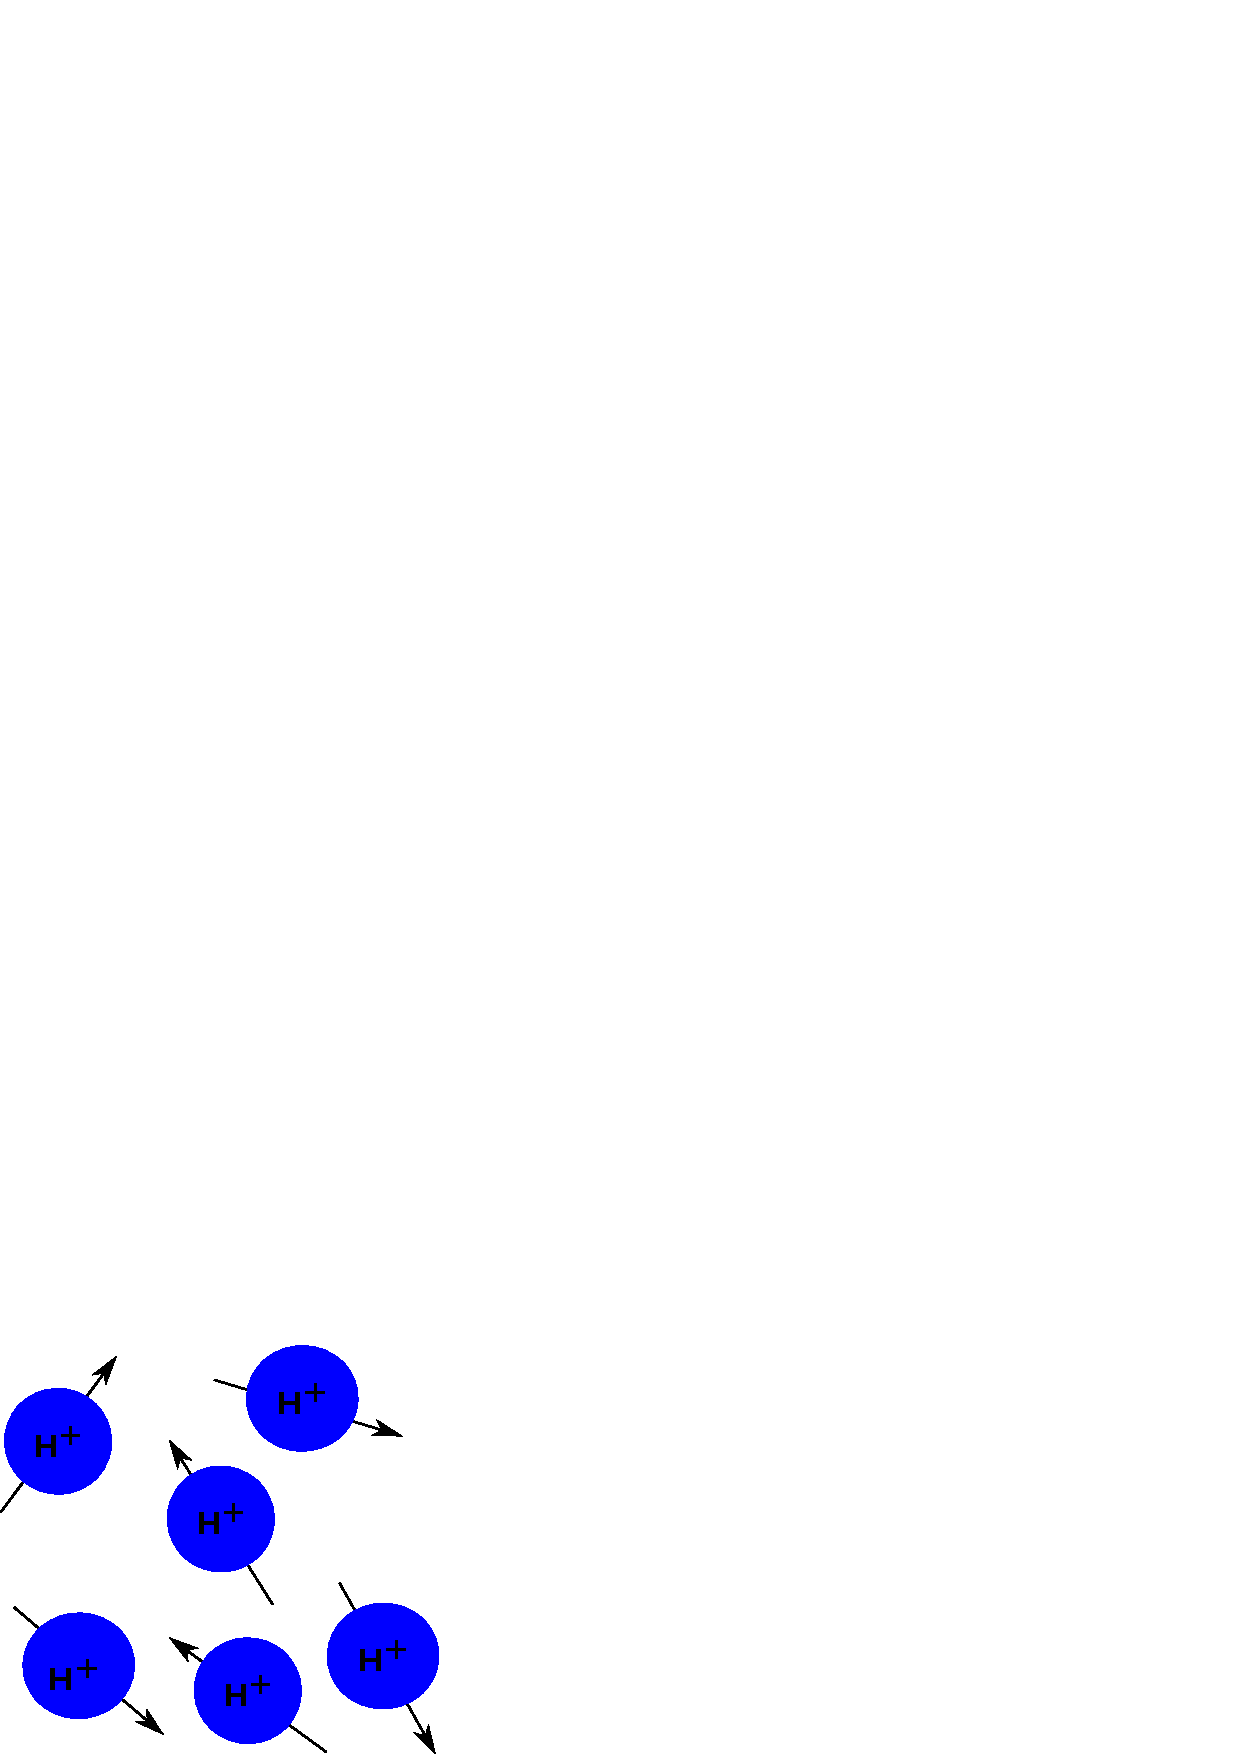
\includegraphics[width=0.75\textwidth]{Images/spins.pdf}
	    \caption{\label{fig:spins}Représentation de noyaux d'hydrogène à l'état de repos.}
    \end{minipage}\hfill
    \begin{minipage}[c]{0.45\textwidth}
	    \centering
	    \includegraphics[width=0.9\textwidth]{Images/spin_b0.pdf}
	    \caption{\label{fig:spin_b0}Représentation de noyaux d'hydrogène dans un champ magnétique $B_0$.}
    \end{minipage}
\end{figure}

Les spins ont alors un mouvement de précession autour de $B_0$ à la fréquence de Larmor $\nu_0$ caractéristique de la particule :
\begin{equation}
    \nu_0 = \frac{\gamma B_0}{2\pi}
\end{equation}
\noindent avec $\gamma=2,675.10^8 \text{ rad}.\text{T}^{-1}.\text{s}^{-1}$ le rapport gyromagnétique propre au noyau d'hydrogène.
Ce mouvement de précession se décompose en deux composantes :
une composante longitudinale suivant l'axe du champ magnétique qui est fixe et une composante transversale qui est en rotation, 
respectivement en jaune et vert sur la \figref{fig:spin_composantes}.

\begin{figure}[ht]
    \begin{minipage}[c]{0.45\textwidth}
	    \centering
	    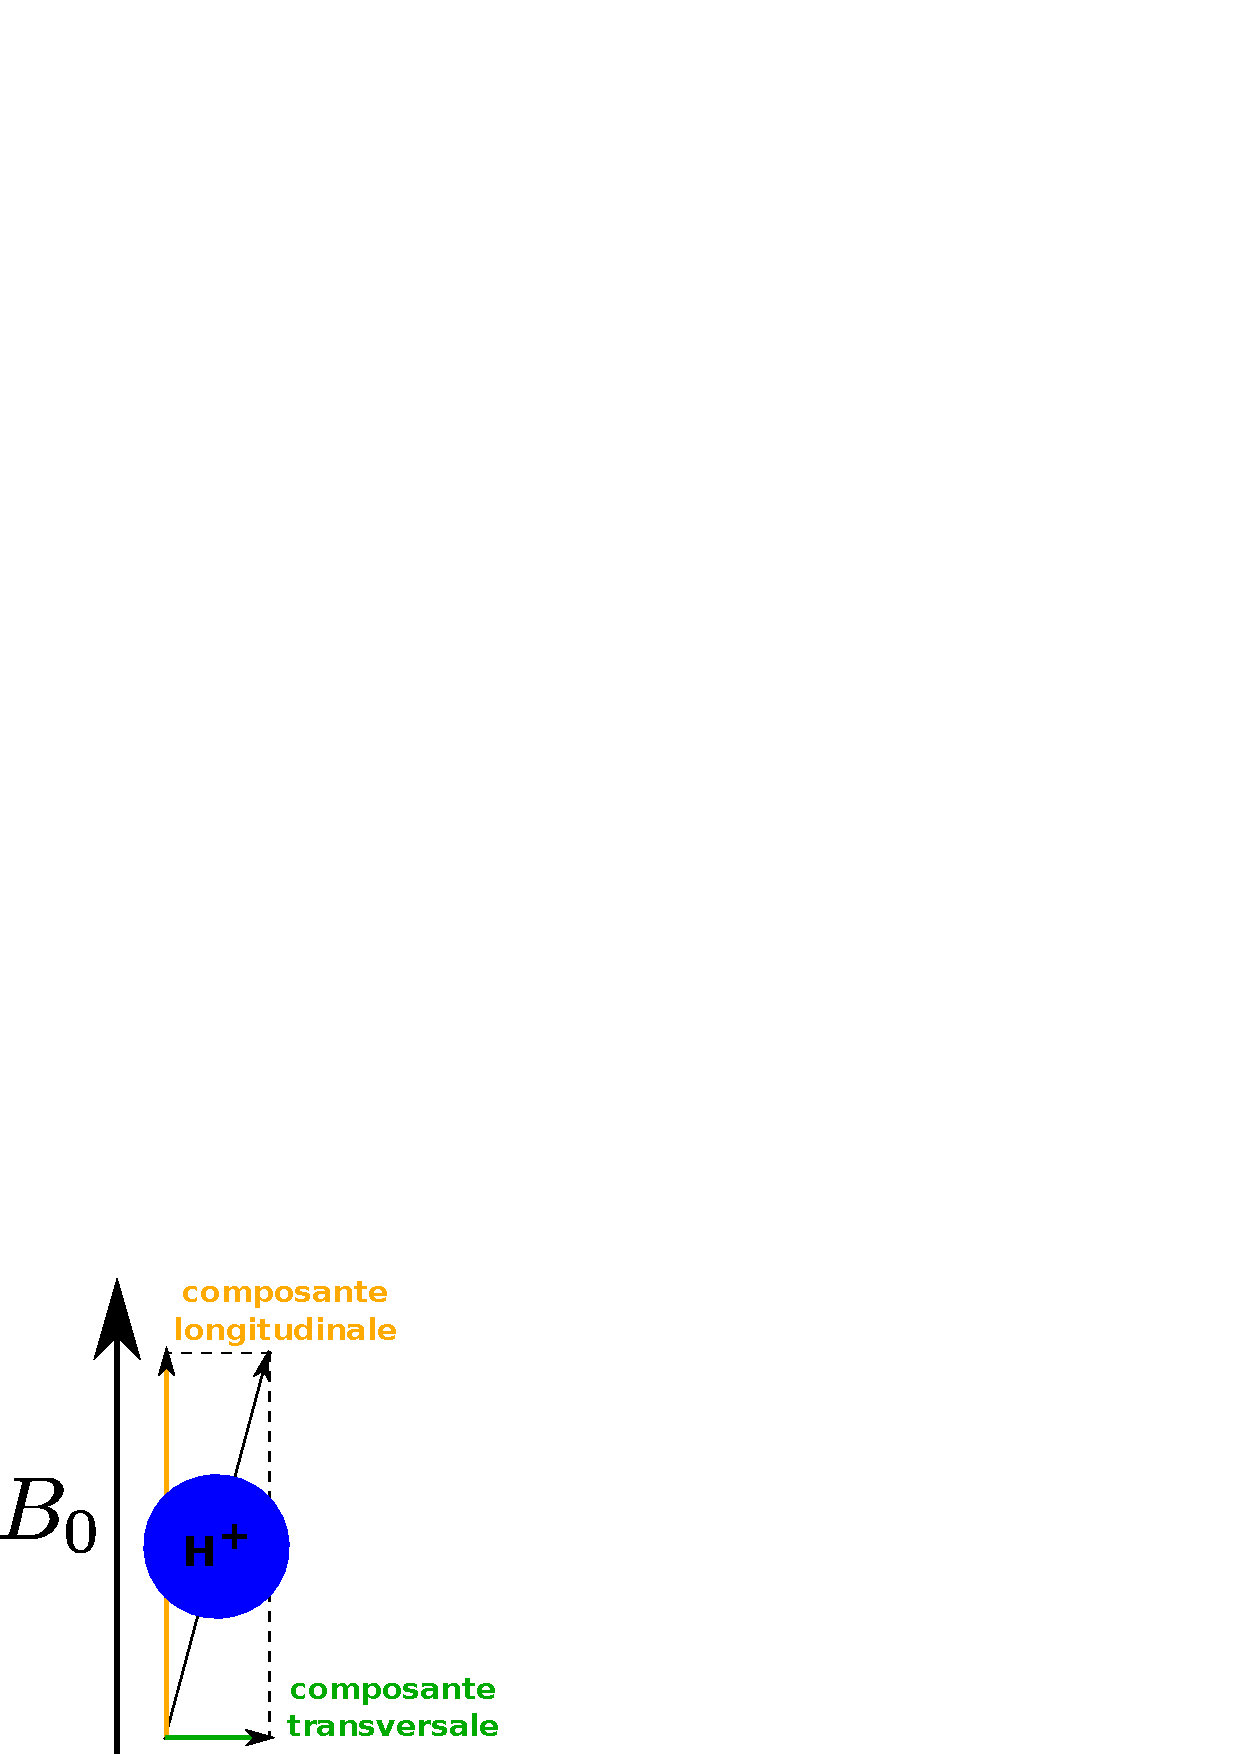
\includegraphics[width=0.7\textwidth]{Images/spin_composantes.pdf}
	    \caption{\label{fig:spin_composantes}Représentation des deux composantes du mouvement de précession d'un noyau d'hydrogène.}
    \end{minipage}\hfill
    \begin{minipage}[c]{0.45\textwidth}
	    \centering
	    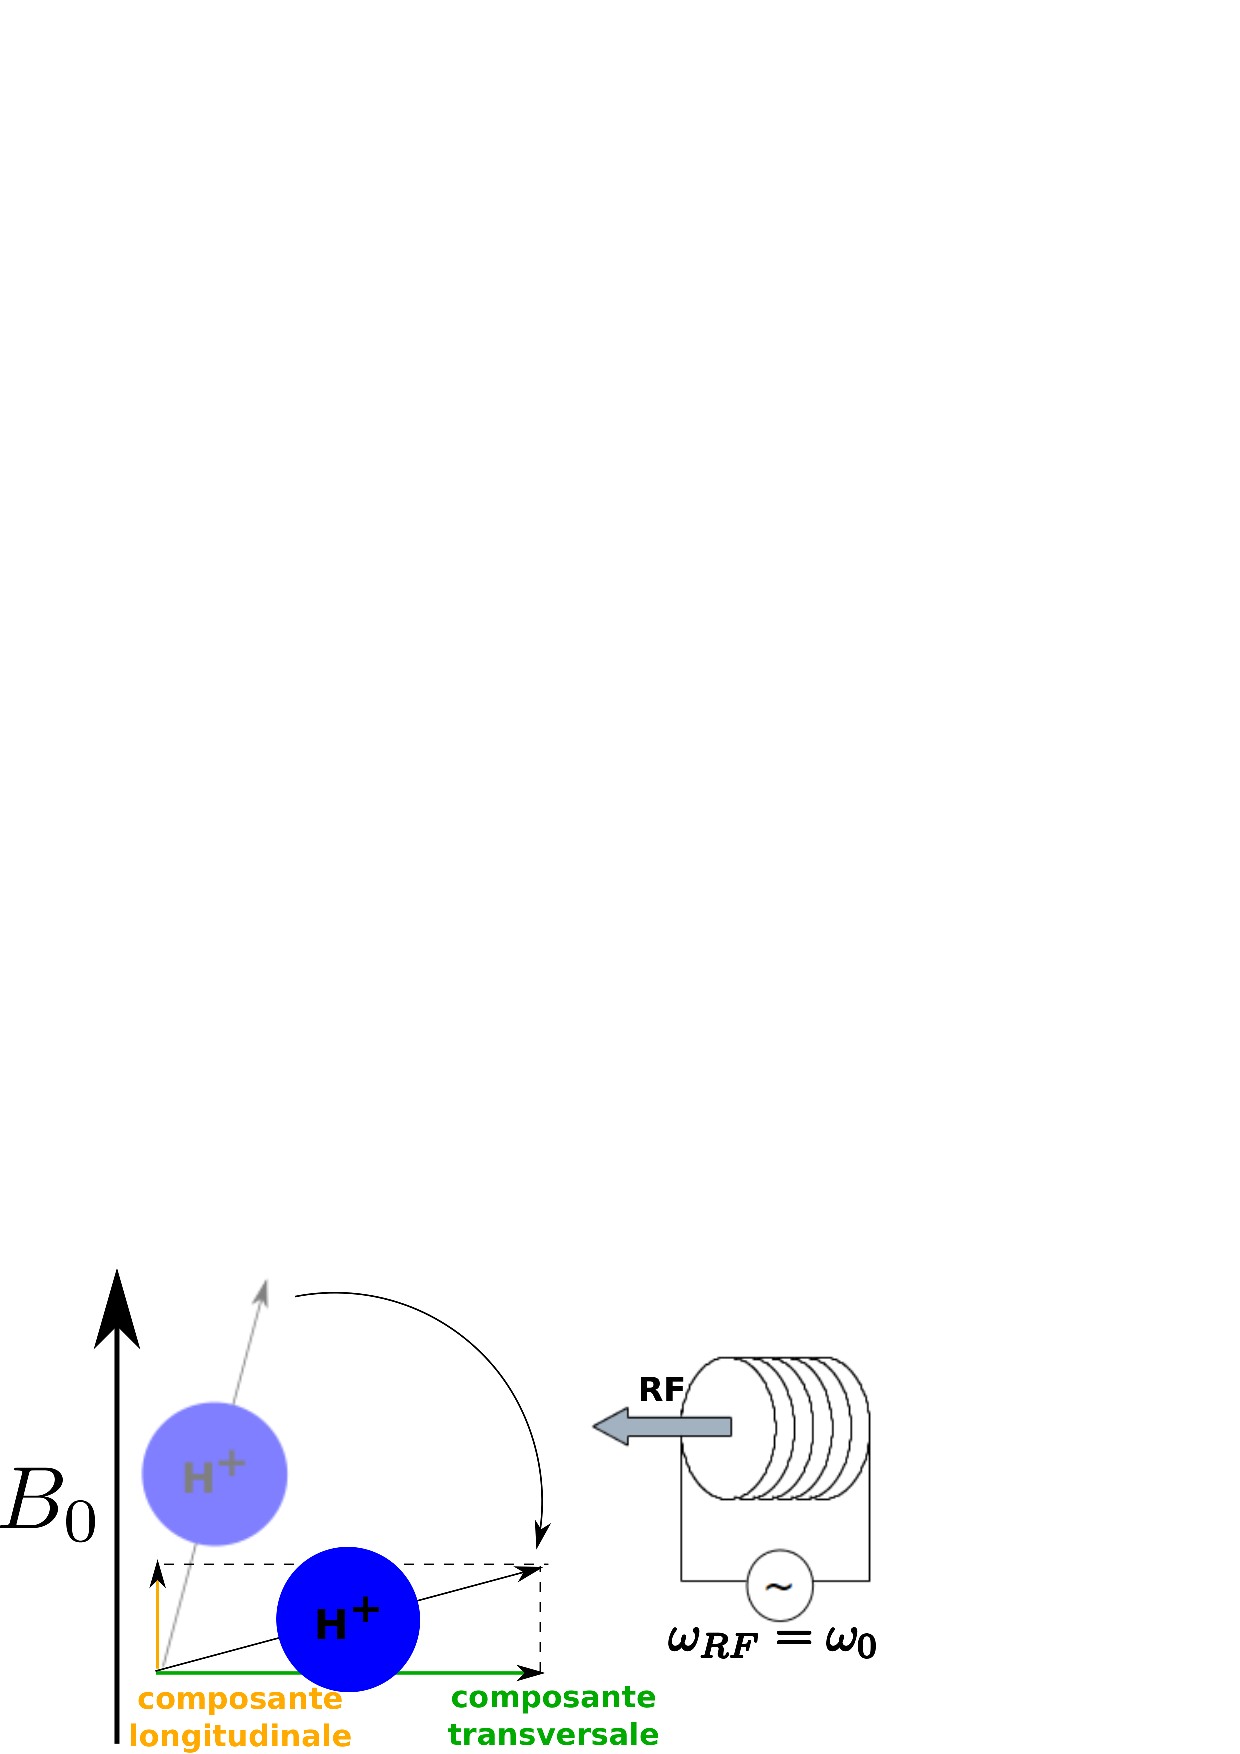
\includegraphics[width=1\textwidth]{Images/excitation.pdf}
	    \caption{\label{fig:excitation}Représentation de la pahse d'excitation.}
    \end{minipage}
\end{figure}

La \rmn consiste à envoyer une onde de Radio-Fréquence (RF) sur ces paticules 
avec une fréquence $\nu_{RF}$ identique à celle de la fréquence de précession $\nu_{0}$.
De cette manière, l'onde RF transmet son énergie aux spins : c'est la phase d'excitation représentée en \figref{fig:excitation}.
Les spins entrent en résonance (\textit{i.e.} ils tournent en phase) et
l'axe de rotation du mouvement de précession bascule.
La composante longitudinale diminue et la composante transversale augmente.
Cette phase d'excitation est suivie par une phase de relaxation durant laquelle les spins retournent à l'état d'équilibre.
Inversement, la composante longitudinale augmente et la composante transversale diminue.
Lors de cette phase, il est possible de mesurer la décroissance de la composante transversale (relaxation $T_2*$)
et avec des séquences particulières, il est possible de mesurer d'autres .

% Lors de cette phase, il est possible de mesurer la décroissance de la composante longitudinale (relaxation $T_1$) 
% ou bien celle de la composante transversale (relaxation $T_2$).
% Lors de cette phase, il est possible de mesurer au cours du temps la composante longitudinale de l'aimantation tissulaire (relaxation $T_1$) 
% ou bien la composante transversale (relaxation $T_2$).

%Ces mesures informent sur l'aimantation globale des tissus.
Pour construire un volume 3D et avoir une valeur par voxel, trois gradients de champ sont utilisés suivant les 3 directions de l'espace. 
Ils servent à la sélection de coupe, au codage en fréquence et au codage en phase.
Les deux derniers gradients définissent la manière dont une matrice $2D$, 
appelée \og espace K \fg, est remplie avec les valeurs de la fréquence spatiale du signal RMN. 
Cette matrice représente ce que nous appelons \og le plan de Fourier \fg et contient les informations pour une seule coupe du volume 3D.
Le module de la transformée de Fourier inverse appliquée à cet espace K permet d'obtenir l'image dans le domaine spatial (signal IRM) 
de la coupe associée (\figref{fig:reconstruction}).
% Une transformée de Fourier inverse est appliquée à cet espace K 
% pour obtenir le signal dans le domaine spatial.
% La magnétude de ce signal permet d'obtenir l'image (signal IRM) de la coupe associée (\figref{fig:reconstruction}).
Le processus est répété pour chaque coupe permettant ainsi de reconstruire le volume 3D.

\begin{figure}[ht]
    \centering
    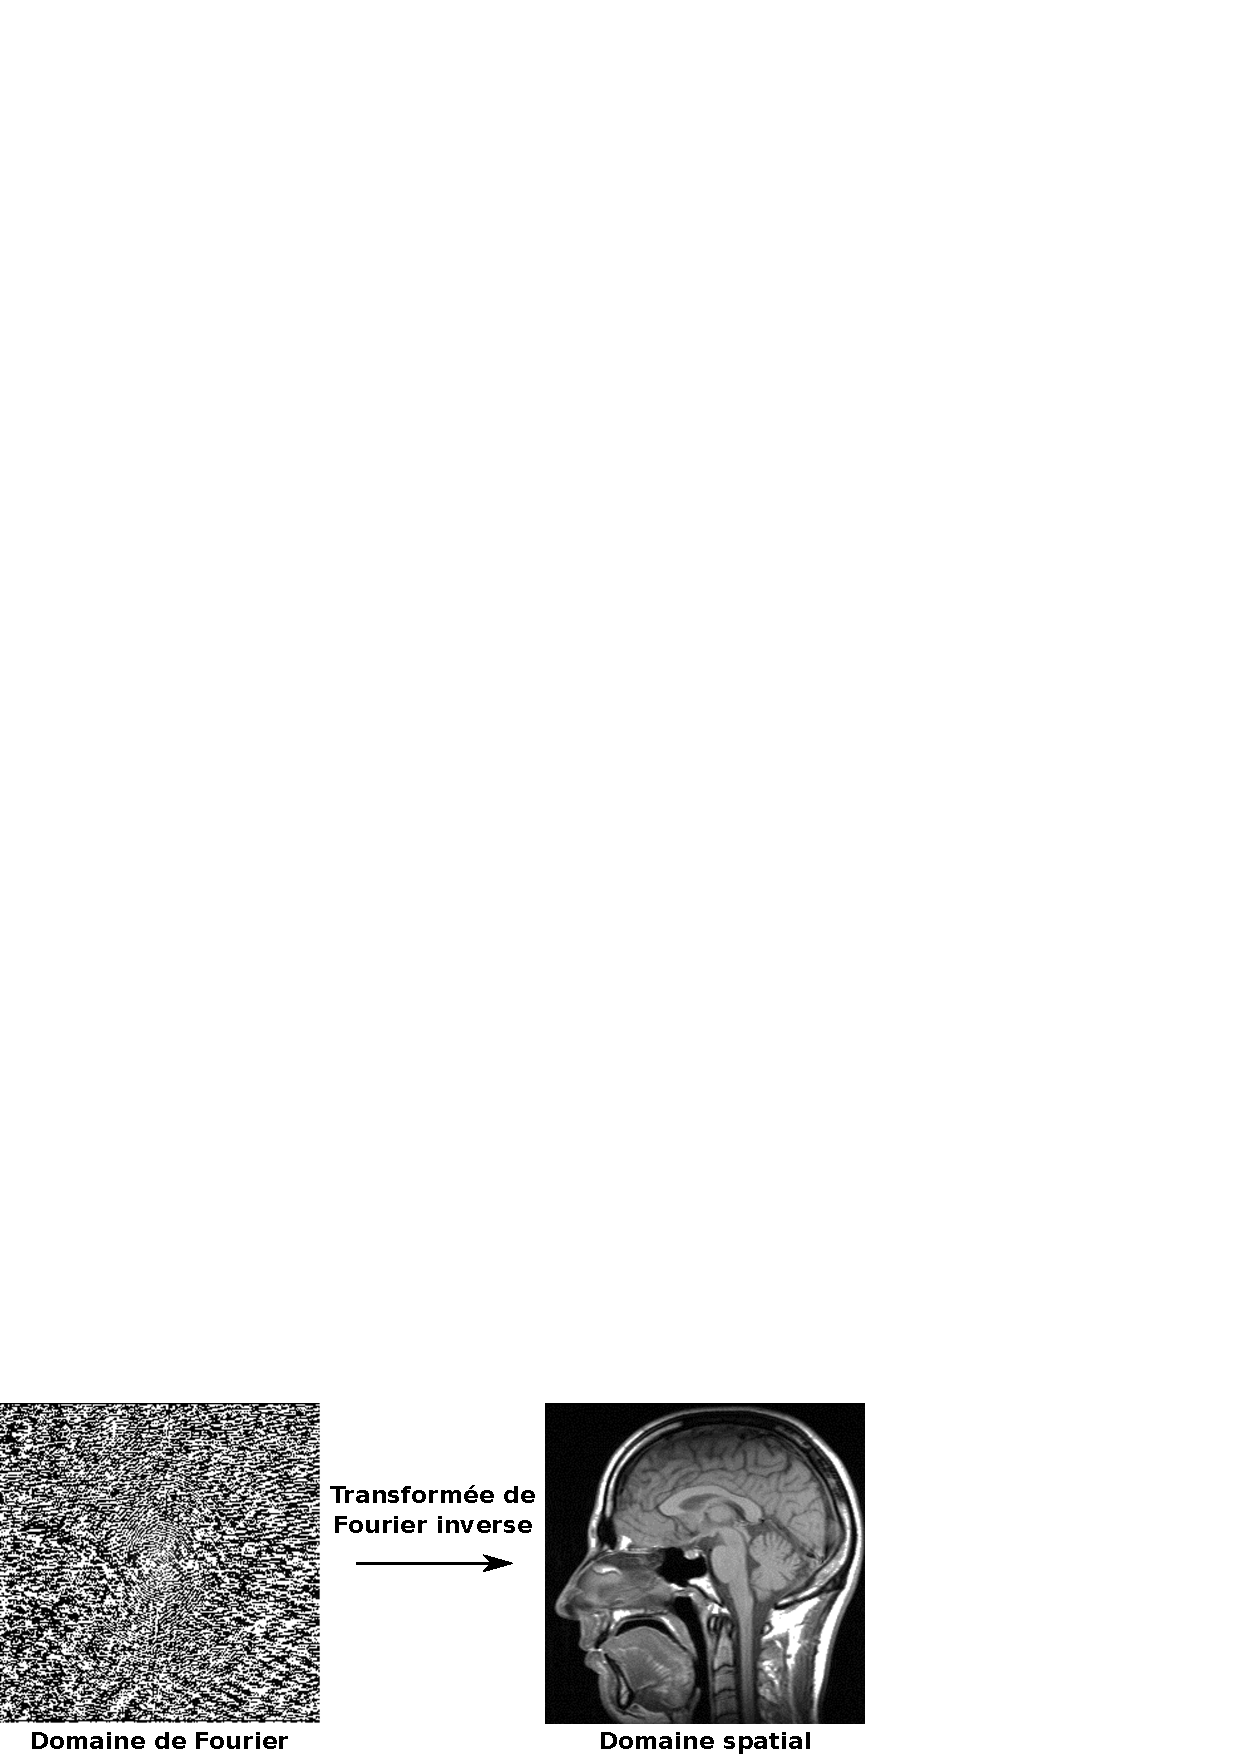
\includegraphics[width=0.8\textwidth]{Images/reconstruction.pdf}
    \caption{\label{fig:reconstruction}Reconstruction d'une coupe 2D à partir du signal acquis dans le domaine de Fourier.}
\end{figure}
Les différentes combinaisons d'ondes RF et de gradients permettent de jouer sur le contraste des tissus, 
la rapidité d'acquisition et l'amélioration du rapport signal sur bruit. 
Cela mène à la création de nouvelles séquences d'acquisition toujours plus performantes.


%\subsection{De la RMN à la diffusion}
%L'\irmd permet de regarder \textit{in vivo} la diffusion des molécules d'eau dans les différents tissus cérébraux.
\subsection{Caractérisation de la diffusion par la RMN}
Ce paragraphe présente la relation entre le principe de la RMN (expliquée précédemment) 
et celui de l'\irmd qui permet de caractériser \textit{in vivo} la diffusion des molécules d'eau dans les différents tissus cérébraux.
Nous commencerons donc par définir le phénomène de diffusion d'une molécule d'eau 
pour aboutir à l'expression liant le signal RMN avec la mesure de la diffusion \eqref{eq:stejskal1965_simple}.\\

Une description rapide du phénomène de diffusion peut être la suivante.
%Le phénomène de diffusion peut être vu de la façon suivante.
Une particule $H^+$ est initialement à la position spatiale $\mathbf{r_0}$.
La probabilité qu'elle se retrouve à la position $\mathbf{r_1}$ après temps $t$ s'écrit $p(\mathbf{r_0}, \mathbf{r_1}, t)$,
souvent notée $p(\mathbf{r}, t)$ avec $\mathbf{r}=\mathbf{r_1} - \mathbf{r_0}$ le vecteur de déplacement.
Cette probabilité, communément appelée \textit{propagateur}, décrit le
déplacement des molécules suivant $I$ directions spatiales $\mathbf{g_{i=0\dots I}}$, 
appelées gradients de diffusion, durant un intervalle de temps $\triangle t$.
Il contient toute l'information relative à la diffusion des molécules d'eau.

En 1965, Stejskal et Tanner \cite{Stejskal1965} mettent en relation le signal acquis par l'IRM $S$
et le propagateur décrivant la diffusion des molécules au cours du temps \eqref{eq:stejskal1965}.
Cette relation montre que le signal $S$ est atténué à cause de l'application des gradients de diffusion : 
les gradients de diffusion déphasent les spins des particules et les rephasent après un durée $\Delta t$ 
au cours de laquelle les particules se sont déplacées spatialement suivant le principe de la diffusion.
À cause de ces déplacements, le rephasage peut ne pas être optimal et cela entraîne un déphasage.
\begin{equation}
    S(\mathbf{g_i},t) = S_0 \int_{voxel} p(\mathbf{r},t)\exp(i\gamma\delta\mathbf{g_i}^T\mathbf{r})d\mathbf{r}
    \label{eq:stejskal1965}
\end{equation}
\noindent avec $S_0$ le signal IRM (acquis sans gradient de diffusion) pondéré en $T_2$, $\gamma$ le rapport gyromagnétique des particules $H^+$ 
et $\delta$ correspondant à la durée d'application du gradient de diffusion.\\

Dans l'équation \eqref{eq:stejskal1965}, l'information de la diffusion est portée par le propagateur $p(\mathbf{r},t)$.
Cependant, c'est une fonction mathématique très complexe attribuant une valeur salaire (probabilité)
depuis un vecteur de déplacements $\mathbf{r}$ et un intervalle de temps $t$ : $p(\mathbf{r},t)\ :\ \mathbb{R}^3\times\mathbb{R} \mapsto \mathbb{R}$.
Cette complexité rend l'analyse de la diffusion difficile.
Dans l'optique de simplifier l'équation \eqref{eq:stejskal1965}, le propagateur peut être modélisé par des outils mathématiques plus simples
tels que le tenseur de diffusion d'ordre 2~\cite{Basser1994} ou d'ordre 4~\cite{Barmpoutis2009} ou les harmoniques sphériques~\cite{Descoteaux2007}.
Dans la littérature, le modèle d'ordre 2 est le plus utilisé.
C'est pourquoi, nous nous sommes basés exclusivement sur ce modèle pour le développement des méthodes.
Nous parlons alors d'Imagerie du Tenseur de Diffusion (ITD).

Cette simplification est faite sous l'hypothèse d'une diffusion libre et non restreinte pour laquelle
le propagateur modélise la diffusion comme un processus gaussien :
\begin{equation}
   p(\mathbf{r}, t) = \frac{1}{\sqrt{(4\pi t)^3 \det(\mathbf{D})}} \exp\left(-\frac{\mathbf{r}^T\mathbf{D}^{-1}\mathbf{r}}{4t}\right)
   \label{eq:diff_gauss}
\end{equation}
\noindent avec $\mathbf{D}$ l'outils mathématique modélisant la diffusion : un tenseur de diffusion d'ordre 2.
Avec cette hypothèse de diffusion gaussienne \eqref{eq:diff_gauss}, 
la relation établie en \eqref{eq:stejskal1965} peut s'écrire sous la forme suivante :
\begin{equation}
    S(\mathbf{g_i}, b) = S_0 \exp\left(-b\mathbf{g_i^T}\mathbf{D}\mathbf{g_i}\right)
    \label{eq:stejskal1965_gauss}
\end{equation}
\noindent avec $b=\gamma^2\delta^2G^2(\Delta t - \frac{\delta}{3})\ (s/mm^2)$ 
la $b$-valeur proportionnelle au temps d'acquisition et $G$ l'amplitude du gradient de sélection de coupe.

En pratique, une séquence d'IRMd acquière une ou plusieurs images $S_0$ pondérées en $T_2$ ($b=0\ s/mm^2$) et 
$I$ images pondérées en diffusion ($b=1000\ s/mm^2$).
Plus la $b$-valeur est élevée et plus l'image acquise est pondérée en diffusion 
mais cela provoque une diminution du rapport signal à bruit.
L'image pondérée en $T_2$ sert de base pour mesurer le tenseur de diffusion 
car elle permet de savoir si un hypersignal mesuré correspond à une diffusion contrainte ou à une particularité anatomique.
La \figref{fig:gradients} représente les différentes images pondérées en diffusion ainsi qu'une image centrale pondérée en $T_2$.

\begin{figure}[ht]
    \centering
    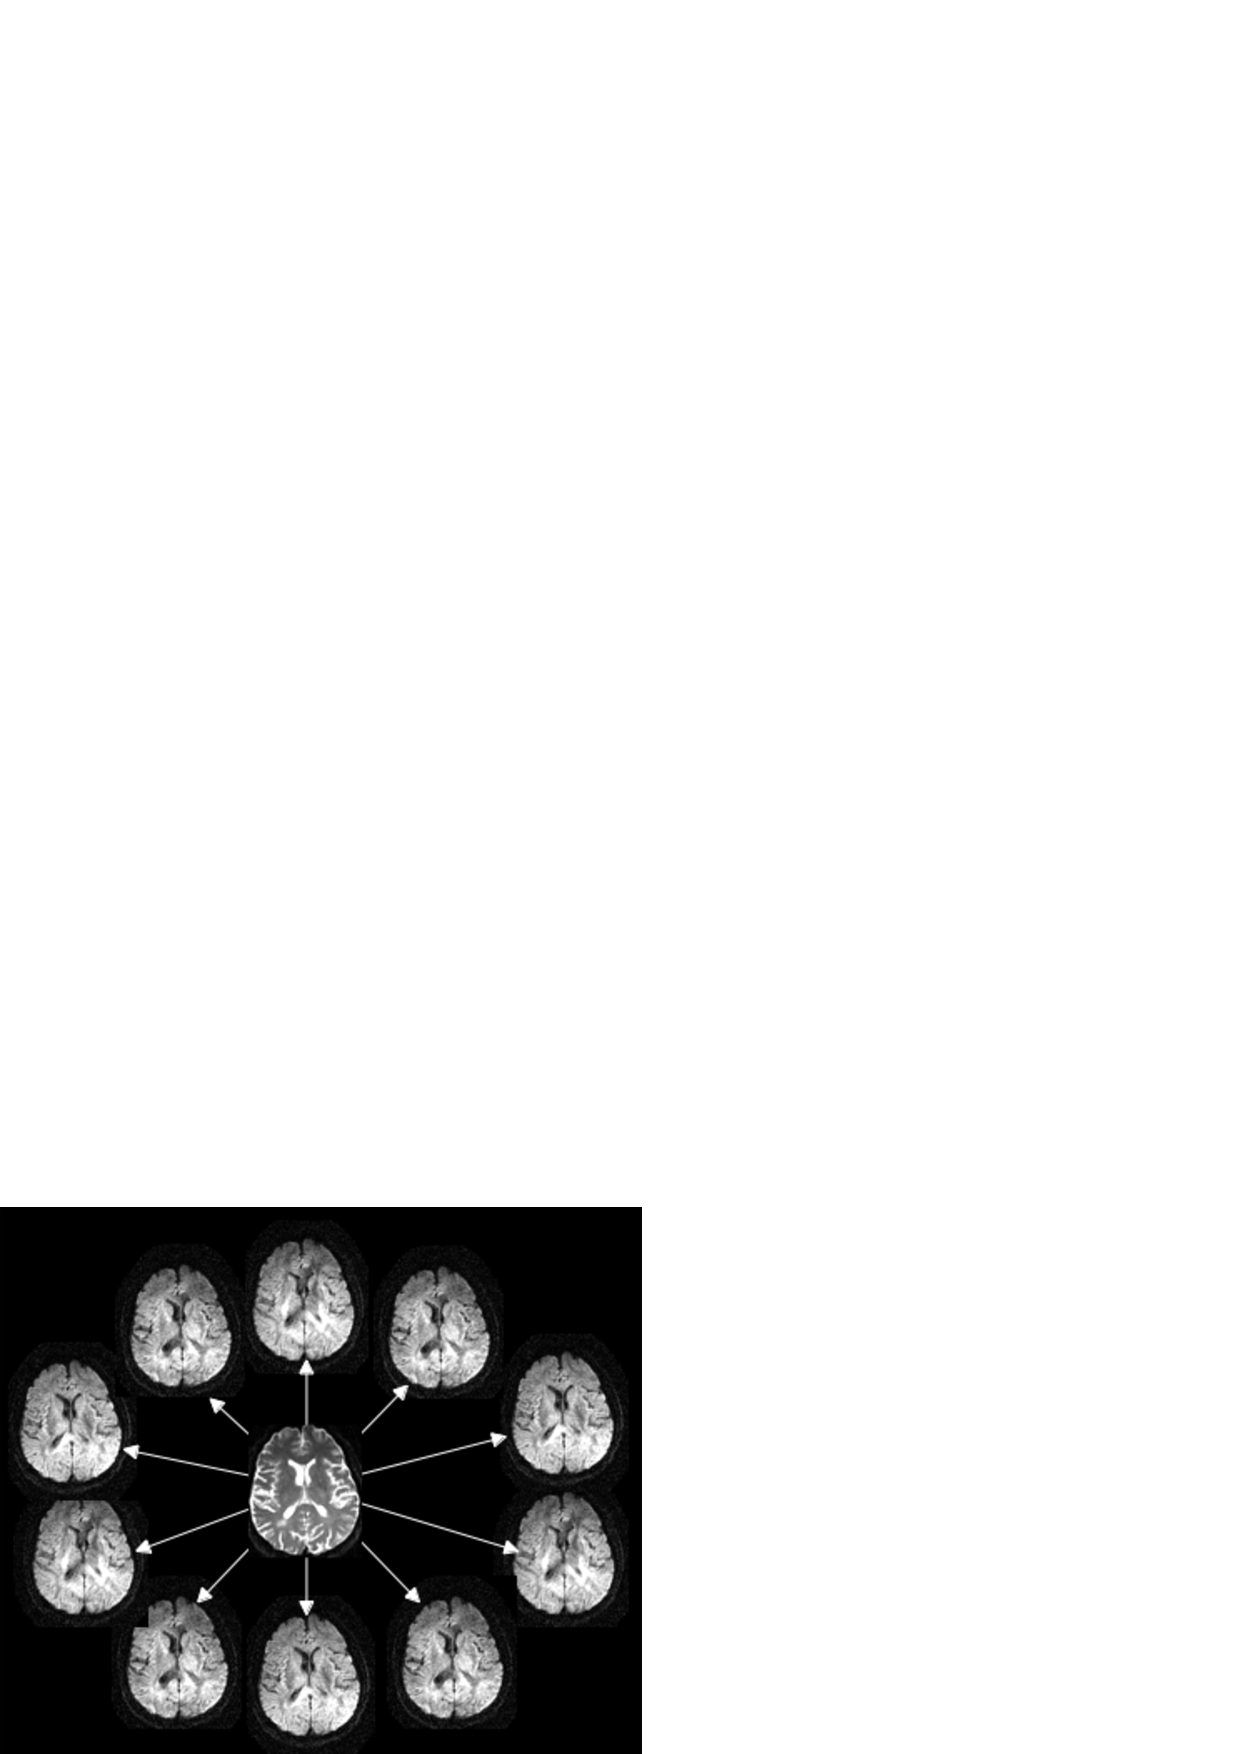
\includegraphics[width=0.5\textwidth]{Images/gradients.pdf}
    \caption{\label{fig:gradients}Les différentes images pondérées en diffusion (images périphériques) 
    et une image pondérée en $T_2$ (image centrale) acquises par une séquence de diffusion.}
\end{figure}

Le terme $\mathbf{g_i^T}\mathbf{D}\mathbf{g_i}$ est un scalaire représentant le Coefficient de Diffusion Apparent ($CDA_i$),
c'est-à-dire la mesure de la diffusion suivant la direction spatiale $\mathbf{g_i}$.
L'écriture de l'équation \eqref{eq:stejskal1965_gauss} peut être simplifiée en notant le signal IRM 
avec gradient de diffusion $S_i$ au lieu de $S(\mathbf{g_i}, b)$.
\begin{equation}
    S_i = S_0 \exp\left( -b \mathbf{g_i^T}\mathbf{D}\mathbf{g_i}\right)
    \label{eq:stejskal1965_simple}
\end{equation}


\section{Tenseur de diffusion}
Dans cette section, nous allons aborder les notions mathématiques fondamentales utilisées pour ce travail de thèse.
Après avoir fait un rappel sur la notion de modèle du tenseur d'ordre 2,
nous verrons comment extraire des indices scalaires représentant certaines informations de la diffusion.
Puis nous verrons la méthode classique d'estimation des tenseurs de diffusion à partir des images pondérées en diffusion.
Enfin, dans un dernier paragraphe, nous présenterons la notion de distance entre deux tenseurs de diffusion ainsi que 
les différentes distances applicables pour des tenseurs d'ordre 2.
% Dans cette section, nous allons aborder les notions mathématiques fondamentales pour comprendre le travail effectué au cours de cette thèse.
% Nous commencerons par faire le point sur la notion de modèle d'ordre 2 
% puis nous verrons comment nous pouvons extraire des indices scalaires représentant certaines informations de la diffusion
% et enfin nous verrons la méthode classique d'estimation des tenseurs de diffusion à partir des images pondérées 
% en diffusion.
% Dans un dernier paragraphe, nous présenterons les différentes distances applicables pour des tenseurs d'ordre 2.\\

Introduit par l'équation \eqref{eq:stejskal1965_gauss}, le tenseur de diffusion $\mathbf{D}$ est un outils mathématique 
qui permet de représenter un objet multi-linéaire, en l'occurence la diffusion de l'eau.
Mathématiquement, un tenseur de diffusion d'ordre $l$ est représenté par un tableau à $p$ dimensions, \underline{défini positif et symétrique}.
Dans la littérature, le modèle d'ordre $l=2$ avec une dimension $p=3$ est le plus fréquemment utilisé~\cite{Basser1994}.
Pour être plus précis, dans le cas de la diffusion, il correspond à la matrice de covariance du déplacement des molécules d'eau.


\subsection{Modèle d'ordre 2}
Le modèle d'ordre 2 du tenseur de diffusion modélise les Coefficients de Diffusion Apparent $CDA_{i=1\dots I}$ sous une forme quadratique \eqref{eq:forme_quatradique}
pour chaque $\mathbf{g_i} = \left[g_{x,i},\ g_{y,i},\ g_{z,i}\right]_{i=1\dots I}$ des $I$ directions de gradients comme vecteurs unitaires.
Cela revient à décomposer le tenseur $\mathbf{D}$ sur une base de polynômes homogènes avec des termes ayant le même degré.
\begin{align}
    CDA_i &= \mathbf{g_i}^T\mathbf{D}\mathbf{g_i} \nonumber \\ 
      &=\sum_{i=1}^{3} \sum_{j=1}^{3} D_{ij}g_ig_j
    \label{eq:forme_quatradique}
\end{align}

Le tenseur de diffusion prend la forme d'une matrice définie positive de dimension 3 avec $3^2$ éléments :
\begin{equation}
    \mathbf{D} = \left[\begin{array}{ccc}
	D_{xx} & D_{xy} & D_{xz}\\
	* & D_{yy} & D_{yz}\\
	* & * & D_{zz}
	\end{array}\right] 
    \label{eq:tenseur_mat}
\end{equation}
\noindent avec $*$ représentant les éléments symétriques de la matrice.

La matrice de diffusion est définie dans le repère physique du scanner IRM $\{\mathbf{x,y,z}\}$.
Il semble plus intéressant de représenter cette diffusion dans un référentiel propre au patient.
Pour cela, une décomposition spectrale \eqref{eq:decomp_spec} permet d'exprimer la matrice $\mathbf{D}$
sur une base de vecteurs propres $\{\mathbf{e_1,e_2,e_3}\}$.
\begin{equation}
    \mathbf{D}\mathbf{e_i} = \lambda_i \mathbf{e_i}
    \label{eq:decomp_spec}
\end{equation}
La transformée de la matrice $\mathbf{D}$ sur cette base est une matrice diagonale 
avec les valeurs propres associées $\{\lambda_1,\lambda_2,\lambda_3\}$ comme éléments diagonaux.
Vu que le tenseur de diffusion est une matrice définie positive à éléments réels et symétrique, 
ses valeurs propres sont positives et réelles.
Ainsi exprimé, le tenseur est représenté dans le repère de la matrice diagonale $\{\mathbf{e_1,e_2,e_3}\}$.

Les vecteurs propres représentent les trois axes de la diffusion avec le vecteur propre $\mathbf{e_1}$
correspondant à la direction principale de la diffusion.
Les valeurs propres sont ordonnées de manière décroissante : $\lambda_1 \geq \lambda_2 \geq \lambda_3$ 
et correspondent à la diffusivité le long de chaque axe respectif.
De cette manière, il est possible de modéliser le phénomène de la diffusion par une ellipsoïde,
comme le schématise la \figref{fig:tenseur}.

\begin{figure}[ht]
    \centering
    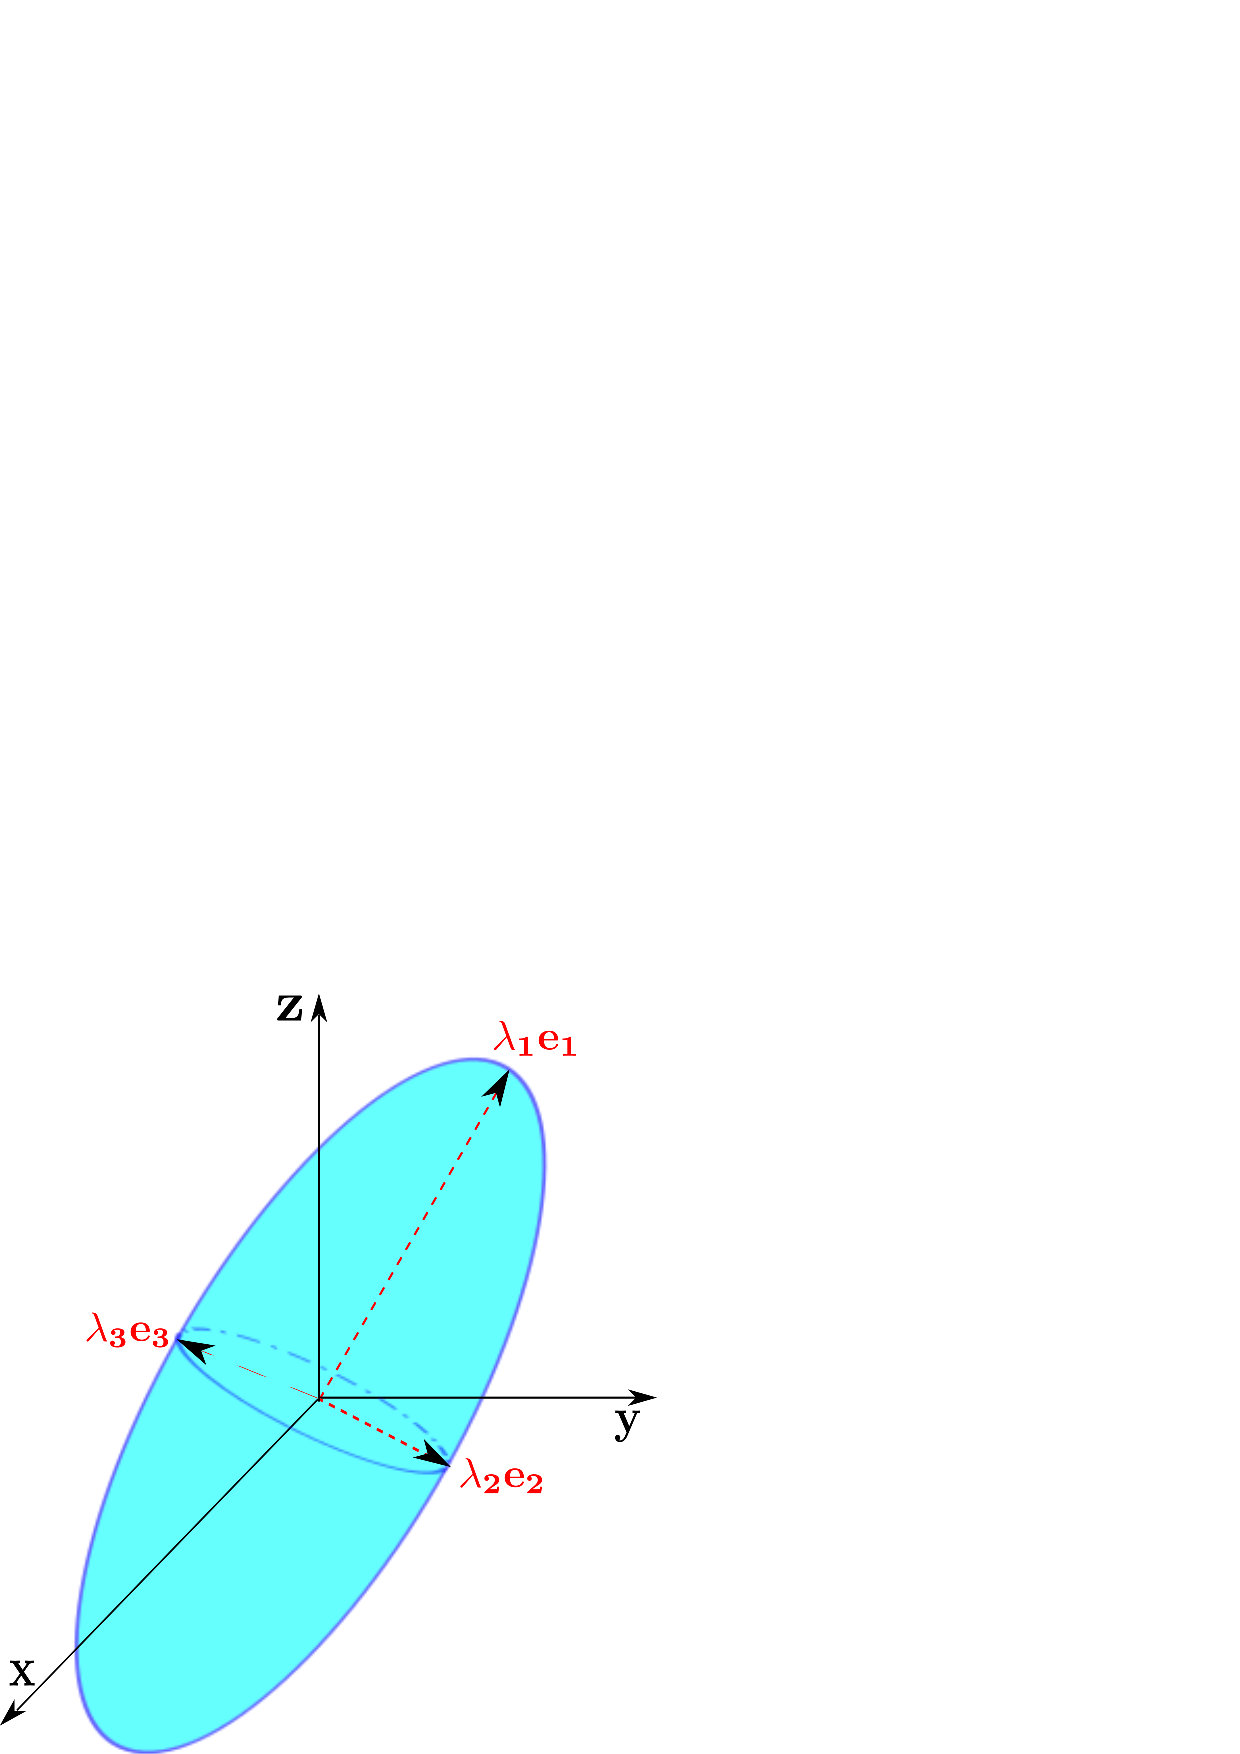
\includegraphics[width=0.4\textwidth]{Images/tensor.pdf}
    \caption{\label{fig:tenseur}Représentation d'un tenseur de diffusion sous la forme d'une ellipsoïde 
    avec le référentiel physique du scanner IRM $\{\mathbf{x,y,z}\}$
    et le référentiel de la matrice diagonale $\{\mathbf{e_1,e_2,e_3}\}$.}
\end{figure}

L'ellipsoïde est définie par trois axes $\{\mathbf{e_1,e_2,e_3}\}$ et trois scalaires $\{\lambda_1,\lambda_2,\lambda_3\}$
qui nous renseigner sur le type de diffusion modélisée.
Il est possible de classer les tenseurs suivant leur forme géométrique définie par les trois scalaires :
\begin{itemize}
    \item les tenseurs à forme sphérique : $\lambda_1 \simeq \lambda_2 \simeq \lambda_3$.
	  Ils dénotent d'une diffusion isotrope: les molécules d'eau se déplacent dans les trois directions de l'espace sans aucune contrainte.
    \item les tenseurs à forme planaire : $\lambda_1 \simeq \lambda_2 \gg \lambda_3$.
	  Dans ce cas, la diffusion est anisotrope car les particules rencontrent une contrainte suivant une des directions.
    \item les tenseurs à forme linéaire : $\lambda_1 \gg \lambda_2 \simeq \lambda_3$.
	  Ces tenseurs sont restreints dans deux des directions de l'espace: ils ont une diffusion dite anisotrope.
\end{itemize}
Pour compléter ce classement sur la diffusion, il est possible, à partir des trois valeurs propres,
de calculer différents paramètres de diffusion que nous appellons \og indices scalaires \fg.
Comme nous le verrons dans le chapitre suivant (\chapref{Chapter2}), l'étude de la forme géométrique d'un tenseur 
peut nous renseigner sur les mécanismes d'une pathologie affectant l'organisation des microstructures cérébrales.


\subsection{Indices scalaires}
Les indices scalaires représentent chacun une unique information sur la diffusion.
Seuls, ils caractérisent partiellement la diffusion, mais vu qu'ils apportent des informations complémentaires,
ils peuvent être combinés et ainsi caractériser totalement la diffusion.\\

Quatre indices scalaires sont les plus souvent utilisés :
\begin{itemize}
    \item La \fa (FA) renseigne sur l'anisotropie de la diffusion. 
    Une valeur de FA grande ($FA=1$) signifie que la diffusion est anisotrope (elle suit un direction privilégiée).
    À l'inverse, une valeur faible de FA correspond à une diffusion isotrope.
    \begin{equation}
        FA = \sqrt{\frac{1}{2}\frac{(\lambda_1 -\lambda_2)^2 + (\lambda_1 -\lambda_3)^2 + (\lambda_3 -\lambda_2)^2 }{\lambda_1^2 + \lambda_2^2 + \lambda_3^2}}
        \label{eq:fa}
    \end{equation}
    \item La \md (DM) indique si la diffusion globale, c'est-à-dire dans les trois directions, est restreinte (DM petite) ou sans contrainte (DM élévée).
    \begin{equation}
        DM = \frac{\lambda_1 + \lambda_2 + \lambda_3}{3}
        \label{eq:md}
    \end{equation}
    \item La \dr (DR) caractérise la diffusion suivant les deux axes secondaires :
    \begin{equation}
	DR = \frac{\lambda_2 + \lambda_3}{2}
        \label{eq:dr}
    \end{equation}
    \item La \da (DA) correspond à la valeur propre associée à la direction principale :
    \begin{equation}
	DA = \lambda_1
        \label{eq:da}
    \end{equation}
\end{itemize}

De nombreux autres indices scalaires peuvent être calculés tels que le mode ou encore l'anisotropie relative.
Cependant, durant la thèse, seuls ces quatre indices scalaires sont utilisés.
La \figref{fig:scalaires} montre trois coupes différentes pour chacun des quatre indices scalaires pour un même sujet.


\subsection{Estimation par les moindres carrés}
L'image contenant en chaque voxel un tenseur de diffusion (modèle d'ordre 2) n'est pas obtenue directement lors d'une séquence d'IRM de diffusion.
Nous avons vu que nous acquierons une série d'images pondérées en diffusion suivant différentes directions.
À partir de cette séquence d'images acquises, il est possible d'estimer les tenseurs de diffusion en chaque voxel du volume 3D.
Nous parlons alors d'\itd (ITD).

La méthode, la plus communément utilisée, est l'estimation au sens des moindres carrés (LS pour \textit{Least Squares}).
Elle permet d'estimer, voxel par voxel, le tenseur d'ordre 2 correspondant.
Elle consiste à résoudre un système linéaire en minimisant l'erreur quadratique entre les données et les estimées.
Pour construire le système linéaire, nous repartons de l'équation \eqref{eq:stejskal1965_simple} 
et nous linéarisons son expression en passant au logarithme.
Nous rappelons qu'il y a $\mathbf{g_{i=1\dots I}}$ gradients de diffusion.
\begin{align}
    \ln \left(\frac{S_i}{S_0}\right) &= -b \mathbf{g_i^T}\mathbf{D}\mathbf{g_i} \nonumber \\
    \ln \left(S_i\right) &= \ln \left(S_0\right) - b \mathbf{g_i^T}\mathbf{D}\mathbf{g_i} \nonumber
\end{align}

La dernière équation peut se réécrire sous la forme matricielle.
Pour un soucis de place, nous avons mis la négation sur les 6 termes du tenseur de diffusion.
\begin{equation}
    \left[\begin{array}{c}
              \ln \left(S_1\right) \\
              \vdots \\
              \ln \left(S_i\right) \\
              \vdots \\
              \ln \left(S_I\right) \\
          \end{array}\right]  = \left[\begin{array}{ccccccc}
				      1 & bg_{1,x}^2 & 2bg_{1,x}g_{1,y} & 2bg_{1,x}g_{1,z} & bg_{1,y}^2 & 2bg_{1,y}g_{1,z} & bg_{1,z}^2\\
				      \vdots & \vdots & \vdots & \vdots & \vdots & \vdots & \vdots \\
                                     1 & b g_{i,x}^2 & 2bg_{i,x}g_{i,y} & 2bg_{i,x}g_{i,z} & bg_{i,y}^2 & 2bg_{i,y}g_{i,z} & bg_{i,z}^2 \\
                                     \vdots & \vdots & \vdots & \vdots & \vdots & \vdots & \vdots \\
                                     1 & b g_{I,x}^2 & 2bg_{I,x}g_{I,y} & 2bg_{I,x}g_{I,z} & bg_{I,y}^2 & 2bg_{I,y}g_{I,z} & bg_{I,z}^2 
                                 \end{array}\right] \left[\begin{array}{c}
							  \ln\left(S_0\right) \\
							  -D_{xx}\\
							  -D_{xy}\\
							  -D_{xz}\\
							  -D_{yy}\\
							  -D_{yz}\\
							  -D_{zz}\\
						      \end{array}\right]	\nonumber
\end{equation}

Nous nous retrouvons face à un système d'équations à 7 inconnues
sous la forme $\mathbf{A} = \mathbf{B}\mathbf{x}$ avec $\mathbf{x}$ le vecteur d'inconnues à estimer.
Pour obtenir une solution à ce système, il est nécessaire d'avoir au minimum $I=7$ équations : 
il faut donc acquérir 7 images pondérées en diffusion avec 7 gradients de diffusion différents. 
La méthode des moindres carrés cherche un solution qui minimise l'erreur quadratique dûe à l'estimation
$\mathbf{\hat{x}} = \arg\min_{\mathbf{x} \in \mathbb{R}^{7}}{\|\mathbf{A} - \mathbf{B}\mathbf{x} \|^{2}}$.
Cela se traduit par une pseudo-inversion matricielle \eqref{eq:pseudoinverse} :
\begin{equation}
    \mathbf{\hat{x}} = (\mathbf{B}^{t}\mathbf{B})^{-1}\mathbf{B}^{t}\mathbf{A}
    \label{eq:pseudoinverse}
\end{equation}

L'\algoref{algo:estimation_tenseur} de cette estimation détaille le pseudo-code implémenté.
\begin{center}
    \begin{minipage}[c]{0.95\textwidth}
	\begin{algorithm}[H]
	    \vspace*{0.5em}
	    \Data{
		$log(S_i) = z_i^t\theta + \epsilon_i$
		$\text{avec  } z_i^t = (1, -b(g_{i,x}^2, 2g_{i,x}g_{i,y}, 2g_{i,x}g_{i,z}, g_{i,y}^2, 2g_{i,y}g_{i,z}, g_{i,z}^2))$
		$\text{et  }\theta = (log(S_0), D_{xx}, D_{xy}, D_{xz}, D_{yy}, D_{yz}, D_{zz})$}\vspace*{1em}
	    \Res{Estimation des 7 paramètres de $\theta$ : $\hat{\theta} = (log(S_0), D_{xx}, D_{xy}, D_{xz}, D_{yy}, D_{yz}, D_{zz})$}\vspace*{1em}
	    \Sortie{$\hat{\theta} = ( \sum_{i=1}^{I} z_i z_i^t )^{-1} \sum_{i=1}^{I} z_i\ log(S_i)$}\vspace*{0.5em}
	    \caption{\label{algo:estimation_tenseur}Estimation du tenseur de diffusion par les moindres carrés}
	\end{algorithm}
    \end{minipage}
\end{center}

Contrairement aux thèses précédentes \cite{Boisgontier_PhD, Grigis_PhD}, nous estimons également l'image $S_0$ pondérée en $T_2$.
De cette manière, lorsque nous rencontrons le cas de multiples images $S_0$, 
la question de savoir s'il faut prendre, pour l'estimation du tenseur, la première de ces images
ou bien faire leur moyenne ne se pose pas.

Cependant, cette estimation (au sens des moindres carrés) présente plusieurs limites.
Premièrement, cette méthode est le meilleur estimateur au sens du maximum de vraisemblance pour un bruit additif gaussien.
Or le bruit de l'acquisition d'un IRM est considéré ricien.
Par conséquent, nous formulons de fortes hypothèses erronées de gaussianité sur les observations en utilisant la méthode des moindres carrés.
Deuxièmement, cette méthode ne garantit pas la positivité des tenseurs.
Différentes solutions à ce problème sont proposées. 
Par exemple, une solution directe et simple en post-estimation consiste à mettre les valeurs propres négatives à 0 
et à reconstruire les tenseurs. 
Ou encore il existe des méthodes d'estimation \cite{Barmpoutis2010} qui prennent en compte la positivité des tenseurs 
mais qui engendrent des calculs de résolution plus complexes.


\subsection{Distances entre deux tenseurs d'ordre 2}
La notion de distance est importante pour la compréhension des travaux de cette thèse.
En effet, le but principal de la compraison de groupes est de regarder 
si la distance entre deux populations de tenseurs de diffusion est statistiquement significative.
Les explications à propos de la compraison de groupe en \itd sont abordées au \chapref{Chapter3}
et un état de l'art sur l'influence du choix de la distance pour mener une comparaison de groupe en ITD est disponible au \chapref{Chapter5}.
Dans ce paragraphe, seules les notions mathématiques relatives aux différentes distances applicables à des tenseurs de diffusion sont présentées.\\

De manière générale, le distance peut être formalisée de la manière suivante :
\begin{adjustwidth}{2cm}{}
    Soit $\mathbb{M}$ une variété et $d:\mathbb{M} \times \mathbb{M} \rightarrow \mathbb{R}^+$ la fonction distance associée à cette variété
    qui vérifie les propriétés suivantes :
    \begin{itemize}
        \item symétrie : $\forall (a,b) \in \mathbb{M}^2, d(a,b)=d(b,a)$
        \item séparation : $\forall (a,b) \in \mathbb{M}^2, d(a,b)=0 \Leftrightarrow a=b$
        \item inégalité triangulaire : $\forall (a,b,c) \in \mathbb{M}^3, d(a,c)\leq d(a,b) + d(b,c)$
    \end{itemize}
    Cette variété est alors un \og espace métrique \fg auquel est rattachée une métrique définissant la distance.
    Suivant la variété, la fonction distance prend une expression mathématique différente.
    En effet, elle mesure la longueur entre deux points appartenant à cette variété en préservant la topologie de l'espace.\\
\end{adjustwidth}

Le tenseur de diffusion d'ordre 2 est une matrice de dimension 3, symétrique et définie positive 
qui peut être associée à trois variétés ayant des topologies différentes :
\begin{itemize}
    \item le domaine Euclidien : $\mathbb{M} \subset \mathbb{R}$,
    \item le domaine Riemannien : $\mathbb{M} \subset Sym^+(3)$,
    \item le domaine Log-Euclidien : $\mathbb{M} \subset Sym(3)$.\\
\end{itemize}

Le domaine Euclidien est un espace vectoriel muni d'un produit scalaire (entre deux matrices)
auquel est associé la norme de Frobenius $\|\mathbf{D}\|=\sqrt{tr(\mathbf{D}^t\mathbf{D})}$.
La distance euclidienne est la norme de Frobenius appliquée à la différence entre deux points du domaine.
\begin{align}
    d_{Euclidien}(\mathbf{D_1}, \mathbf{D_2}) &= \|\mathbf{D_1}-\mathbf{D_2} \| \nonumber \\
    &= \sqrt{tr((\mathbf{D_1}-\mathbf{D_2})^t(\mathbf{D_1}-\mathbf{D_2}))}
\end{align}
Cependant, même si cette distance entre deux réels permet d'obtenir un réel,
lorsqu'elle est appliquée à deux matrices symétriques définies positives, 
elle n'assure pas la positivité du résultat et seule la symétrie est conservée.\\

Ce problème est résolu lorsque la distance Riemannienne \cite{Pennec2006, Fletcher2007} est utilisée.
L'espace Riemannien est un espace courbé, représenté sur la \figref{fig:sphere} par une sphère.
La distance entre deux points de cet espace est un chemin géodésique qui respecte la topologie de l'espace (courbure).
\begin{equation}
    d_{Riemannien}(\mathbf{D_1}, \mathbf{D_2}) = \sqrt{\frac{1}{2} tr\left(\log \left(\mathbf{D_1}^{-\frac{1}{2}}\mathbf{D_2}\mathbf{D_1}^{-\frac{1}{2}} \right)^2 \right)}
\end{equation}


Cependant, d'un point de vue implémentation, cette distance demande des opérations complexes qui peuvent se révéler consommatrices en temps de calcul.
Pour éviter ce désavantage, une nouvelle distance a été définie : la distance Log-Euclidienne \cite{Arsigny2006}.
Elle prend la forme d'une application projetant le tenseur de l'espace $Sym^+(3)$ sur un plan tangent Euclidien (\figref{fig:log_sphere}).
À partir de là, les métriques du domaine Euclidien peuvent être appliquées sur le tenseur projeté.
\begin{align}
    d_{Log-Euclidien}(\mathbf{D_1}, \mathbf{D_2}) &= \|\log \left(\mathbf{D_1}\right)- \log \left(\mathbf{D_2}\right) \|
\end{align}



\begin{figure}[ht]
    \begin{minipage}[c]{0.4\textwidth}
	    \centering
	    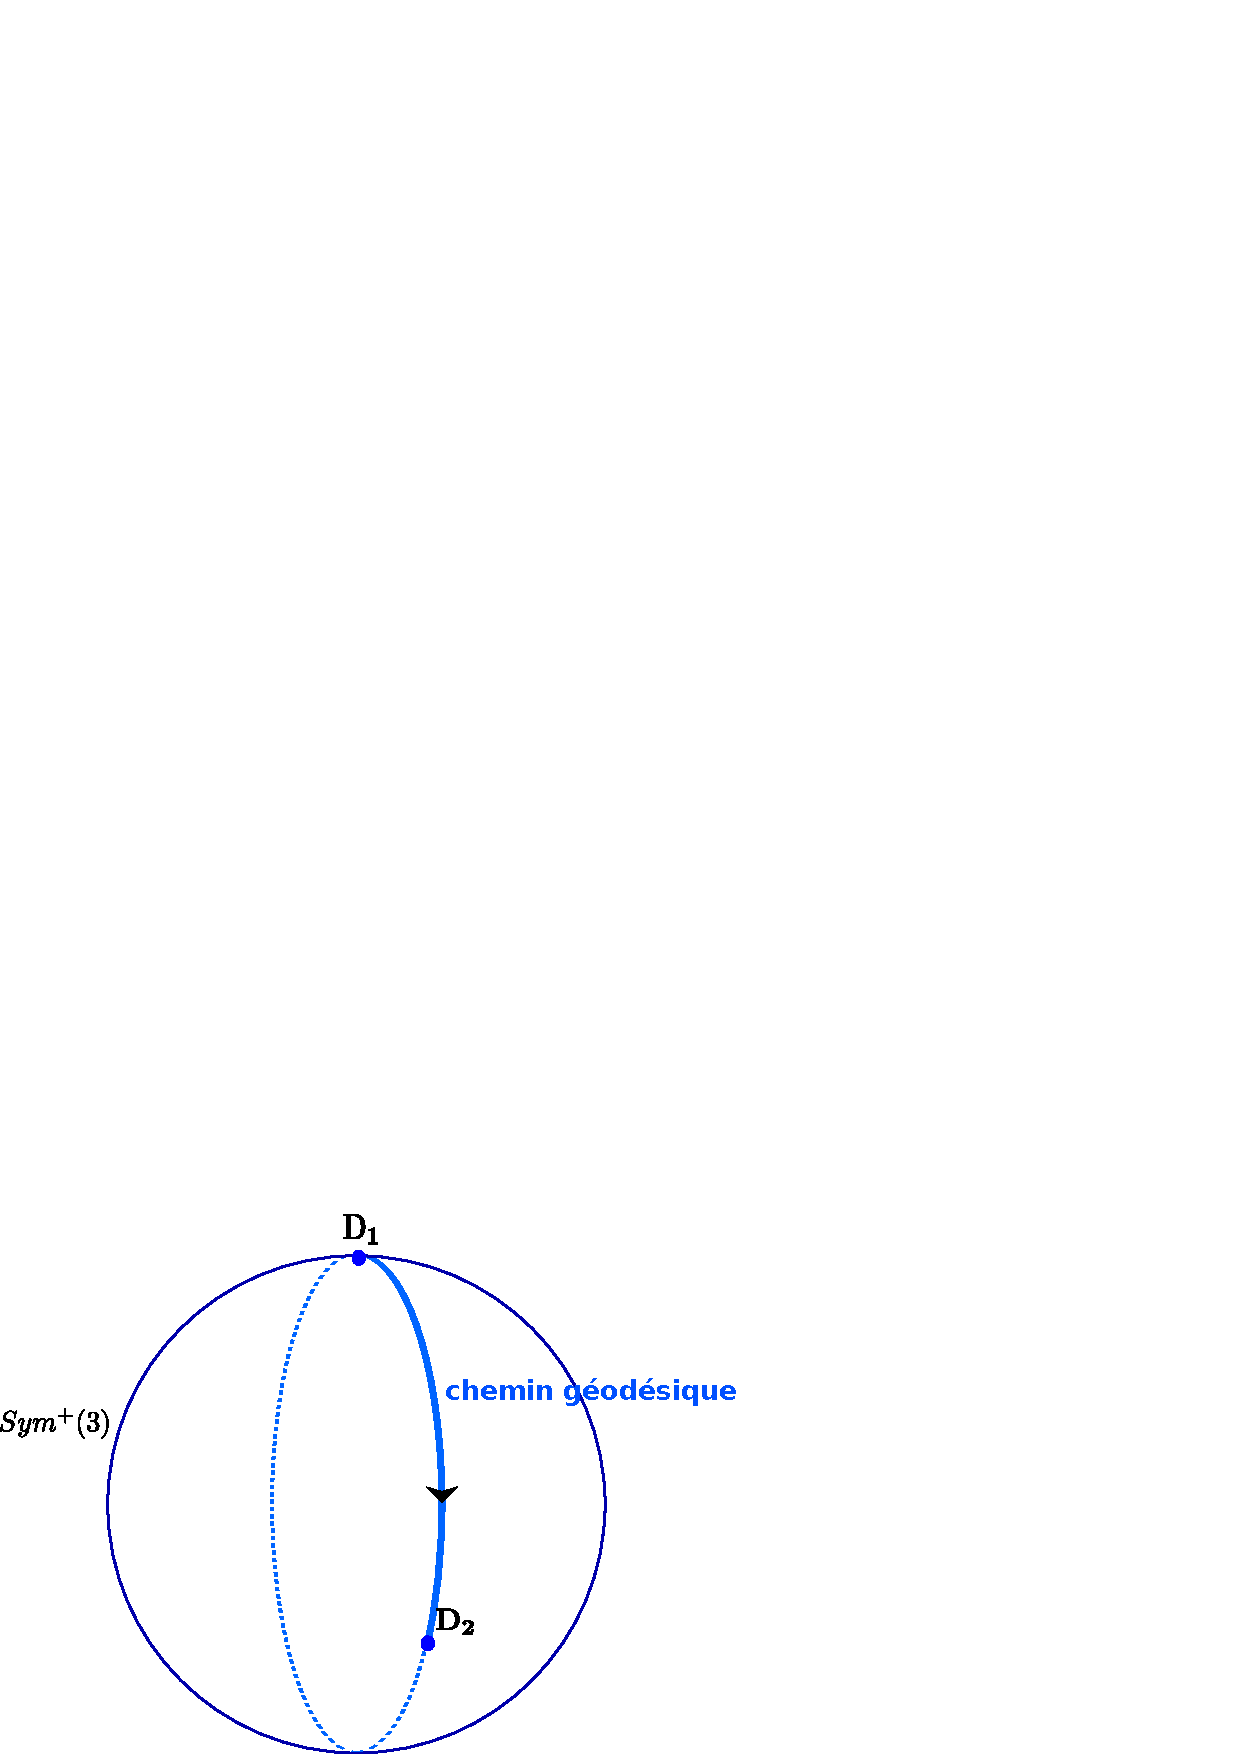
\includegraphics[width=0.85\textwidth]{Images/sphere.pdf}
	    \caption{\label{fig:sphere} Illustration de l'espace Riemannien sous forme de sphère.}
    \end{minipage}\hfill
    \begin{minipage}[c]{0.5\textwidth}
	    \centering
	    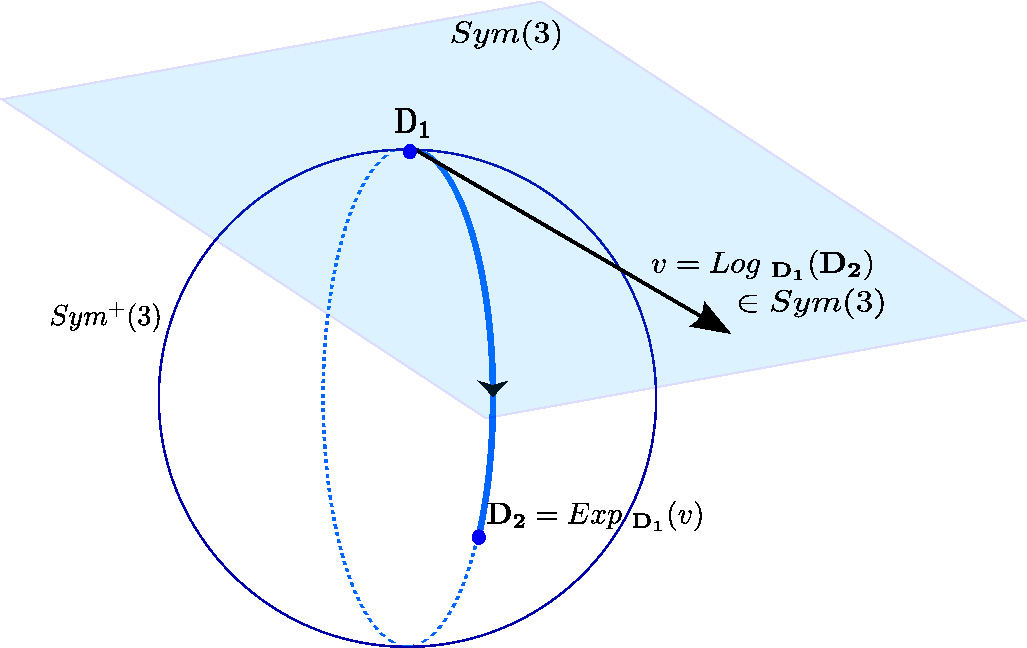
\includegraphics[width=1\textwidth]{Images/log_exp_map_sphere.pdf}
	    \caption{\label{fig:log_sphere} Illustration de l'espace Riemannien avec un plan tangent.}
    \end{minipage}
\end{figure}


\begin{figure}[ht]
    \centering
    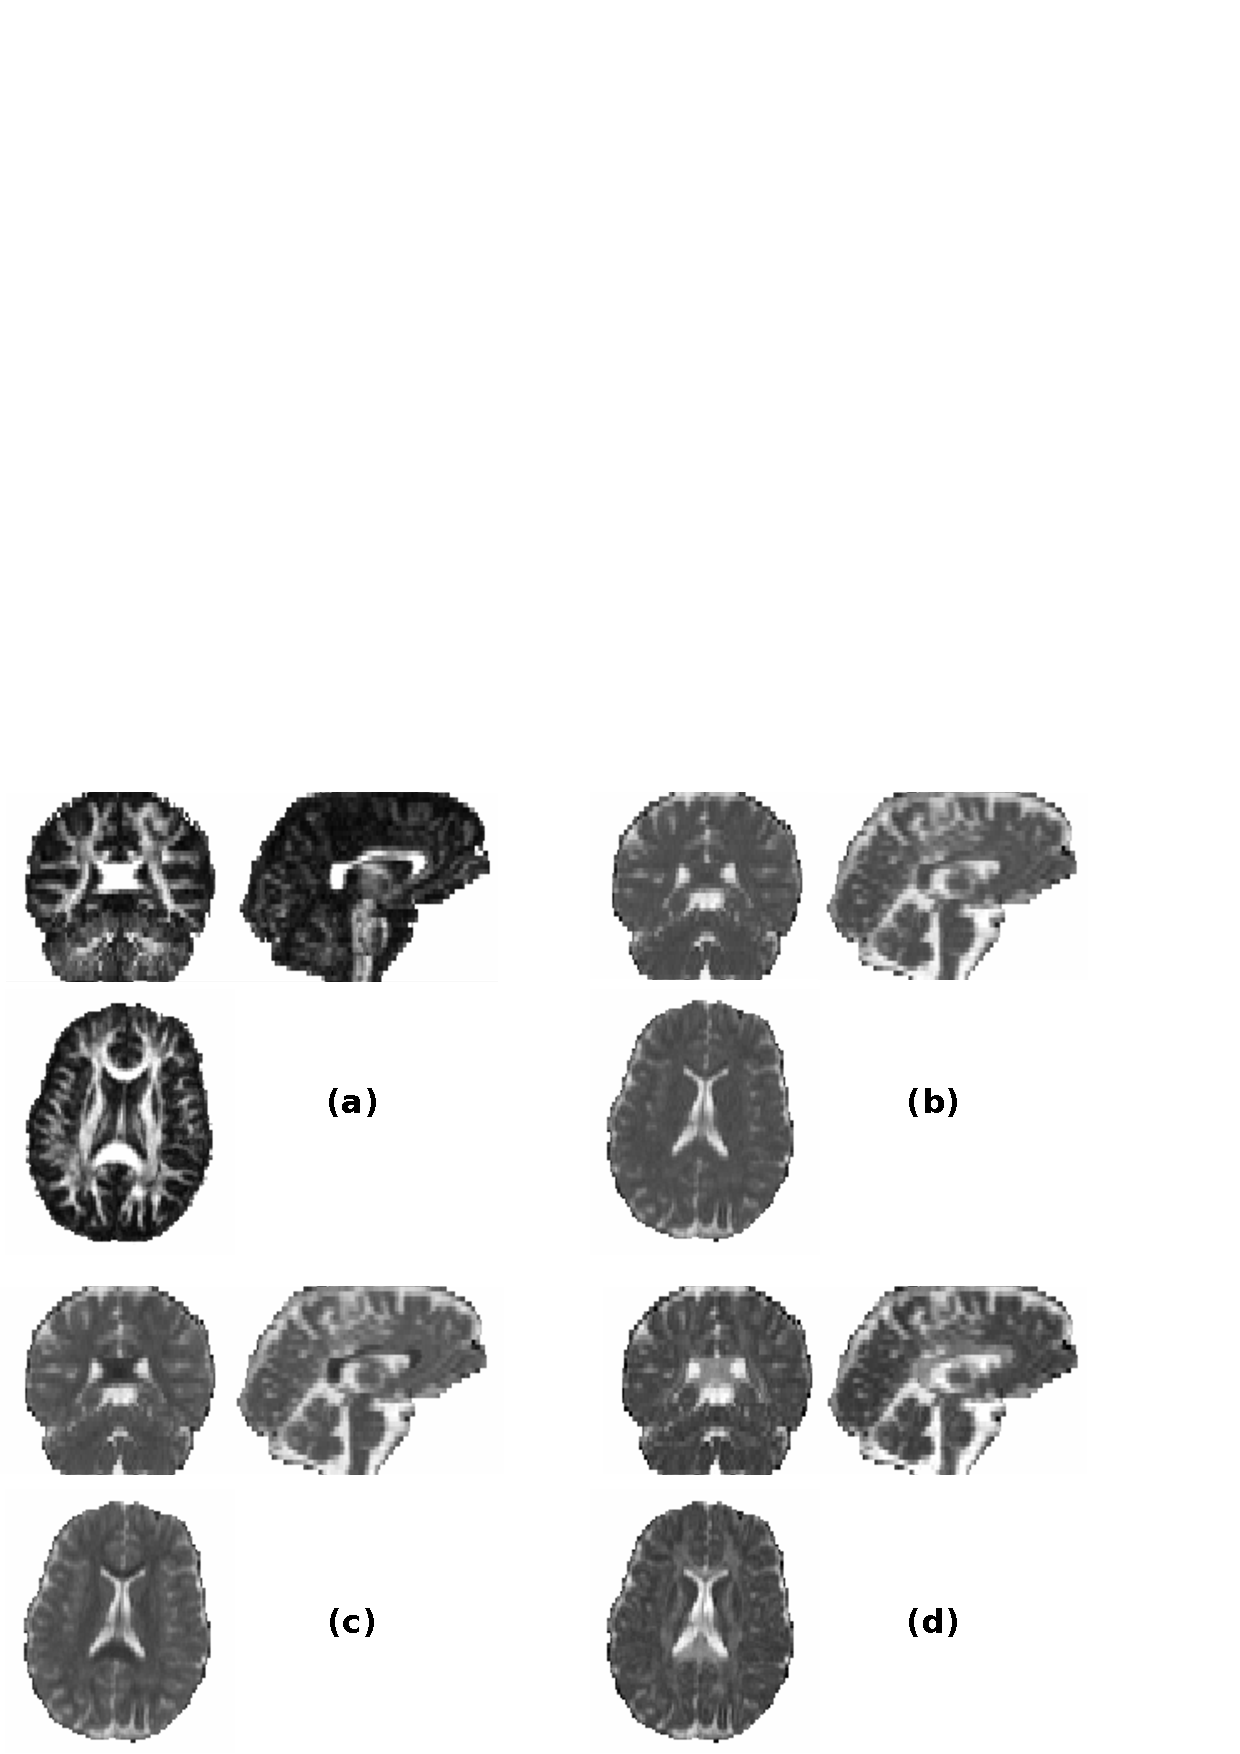
\includegraphics[width=1\textwidth]{Images/scalaires.pdf}
    \caption{\label{fig:scalaires}Images des indices scalaires pour un sujet : \textbf{(a)} FA, \textbf{(b)} DM, \textbf{(c)} DR, \textbf{(d)} DA.}
\end{figure}


    %%%%%%%%%%%%%%%%%%%%%%%%%%%%%%%%%%%%%%%%%%%%
% Chapitre 2
%%%%%%%%%%%%%%%%%%%%%%%%%%%%%%%%%%%%%%%%%%%%


\chapter{La diffusion pour la médecine}
\label{Chapter2}

    
      % partie 2
    \part{Méthodes de comparaison de deux populations de tenseurs de diffusion}
    \label{Part2}
    %%%%%%%%%%%%%%%%%%%%%%%%%%%%%%%%%%%%%%%%%%%%
% Chapitre 3 - INTRO
%%%%%%%%%%%%%%%%%%%%%%%%%%%%%%%%%%%%%%%%%%%%

\chapter*{Introduction}
\markboth{\textbf{Introduction}}{}
%---------------------------------------------------------------------------------------

    %%%%%%%%%%%%%%%%%%%%%%%%%%%%%%%%%%%%%%%%%%%%
% Chapitre 3
%%%%%%%%%%%%%%%%%%%%%%%%%%%%%%%%%%%%%%%%%%%%

\chapter{Comparaison de groupes}
\label{Chapter3}

La comparaison de groupes consiste à chercher les changements, statistiquement significatifs, entre deux populations d'observations. 
En imagerie médicale, cela revient dans la plupart des cas d'étude, à comparer une population de sujets atteints d'une pathologie avec une population de sujets sains afin de mettre en avant les zones affectées par la maladie.
Cette méthode mathématique comporte deux parties centrales de traitements : la régression et l'analyse statistique. 
La première permet d'expliquer les observations grâce à des variables explicatives connues et associées à chaque observation, ainsi qu'à des régresseurs à estimer pour chacun des deux groupes.
La deuxième partie sert à tester si ces régresseurs présentent une différence statistiquement significative.
Ces parties sont généralement précédées par des pré-traitements tels que la correction des artefacts d'acquisition, le recalage et le fitrage.\\

% \minitoc

%----------------------------------------------------------------------------------------

\section{Contexte}
La comparaison de groupes s'inscrit dans un contexte de recherche pure. 
Il n'y a aucune application directe du praticien à son patient en clinique.
Par contre, les aboutissements d'une telle méthode apportent au médecin, une meilleure compréhension du mécanisme de la pathologie et une aide au diagnostique et au pronostique.
Les utilisateurs de cette approche sont aussi bien des scientifiques travaillant à résoudre les différents problèmes rencontrés (voir Section \ref{problematiques}) que des médecins analysant les résultats obtenus par des logiciels tels SPM ou SnPM\footnote{\url{http://warwick.ac.uk/snpm}}.

D'un point de vue parenté, cette méthode s'apparente à la comparaison longitudinale de deux images de tenseur consécutives d'un même patient \cite{Grigis2012}.
Le fait de prendre deux populations de sujets plutôt que seulement deux images longitudinales permet de réduire la variabilité inter-individus. 
Comme conséquence, cette approche rend le système statistique plus puissant pour détecter les zones de changements entre les deux groupes et non plus les variations structurelles d'un individu à un autre.

De plus, il est à noter que les cohortes ont des tailles de plus en plus importantes.
Comme exemples de base de données aux échelles nationale et internationale, Baltazar\footnote{\url{https://clinicaltrials.gov/ct2/show/study/NCT01315639?term=baltazar&rank=1}}, ADNI\footnote{\url{http://adni.loni.usc.edu/}} ou encore OSEP\footnote{\url{http://www.ofsep.org/fr/}} peuvent être citées.
La grande taille des échantillons dans un modèle statistique est un atout car cela rend les résultats obtenus plus fiables.


\section{Problématiques}
\label{problematiques}
Dans cette section, les différents problèmes intrinsèques à la comparaison de groupes seront abordés.
Trois axes principaux ont été dégagés et sont exposés dans l'ordre suivant : 
les problématiques liées à la multivariabilité des données, les problématiques provenant de la pré-étape de recalage et
les problématiques dûes à la géométrie du tenseur de diffusion.
Les travaux de cette thèse ont consisté à apporter des réponses ou encore à évaluer l'influence de ces trois points.

\subsubsection*{Problématique liée à la dimension des données}
Ce paragraphe n'est pas un état de l'art. 
Il sert simplement à introduire aux lecteurs les problèmes rencontrés à cause de la dimension des données.
Un état de l'art détaillé est proposé dans la prochaine section (voir \secref{etat_art}).\\
La multi-dimensionnalité des données est le problème majeur des images du tenseur de diffusion autant pour les pré-traitements que pour les traitements. 
Les tenseurs s'expriment sous forme de matrice de dimension 3, symétrique et définie positive, $D \in Sym^{+}(3)$~\cite{Basser1994} :
\begin{center}
    $\textbf{D} = \left[\begin{array}{ccc}
    D_{11} & D_{12} & D_{13}\\
    * & D_{22} & D_{23}\\
    * & * & D_{33}
    \end{array}\right]$
\end{center}
Toutes les informations permettant de décrire globalement la diffusion en un voxel, sont contenus dans cette matrice : 
diffusion radiale et axiale, orientation de la diffusion, diffusion moyenne ou encore fraction d'anisotropie.
Comme expliqué en début de chapitre, la comparaison de groupes consiste en deux opérations mathématiques : la régression et l'analyse statistique.
Elles peuvent être sous-divisées en opérations simples telles que l'addition, la soustraction, la division, la somme, la puissance ...
Ces opérations s'appliquent très facilement sur des scalaires.
Cependant appliquer une de ces opérations sur les images de tenseur de diffusion, revient à faire du calcul matriciel ce qui peut considérablement compliquer la tâche.
De plus, les hypothèses statistiques nécessaires pour la régression et l'analyse statistique peuvent totaltement différer entre le scalaire et la matrice.\\
Plusieurs techniques sont possibles pour traiter ce type de données. 
La première, la plus utilisée, consiste à extraire des scalaires (FA ou MD) de la matrice et à appliquer les méthodes de détection directement sur ces scalaires.
Deuxièment, des méthodes proposent de s'occuper seulement des 6 éléments supérieurs de la matrice en les concatenant dans un vecteur.
\begin{center}
    $vect(\textbf{D}) = \left[\begin{array}{cccccc}
    D_{11} & D_{12} & D_{13} & D_{22} & D_{23} & D_{33}
    \end{array}\right]^{T}$
\end{center}
Troisièment, certaines techniques s'appliquent directement sur la matrice entière du tenseur de diffusion.
%%%%%%%%%%%%%%%%%%%%%%%%%%%%%%%%%%%%%%%%%%%%%%%%%%%%%%%%%%%%%%%%%%%%%%%%%%%%%%%%
\subsubsection*{Problématique liée à la géométrie de l'espace des tenseurs}
Comme expliqué au \chapref{Chapter1}, page \pageref{Chapter1} du manuscrit, un tenseur de diffusion $\textbf{D}$ 
est représenté mathématiquement par une matrice de dimension 3, symétrique et définie positive, $\textbf{D} \in Sym^{+}(3)$~\cite{Basser1994}.
La définition positive du tenseur se vérifie si toutes ses valeurs propres sont strictement positives.
Cette géométrie particulière implique que l'espace du tenseur n'est pas un espace Euclidien mais un cône convexe défini dans cet espace vectoriel. 
Dans ce sous-espace, des métriques de l'espace Euclidien restent stables mais elles n'imposent aucune contrainte sur la positivité des tenseurs.
Certaines opérations entrainent des valeurs propres nulles ou négatives.
Prenons comme exemple simple, le résultat de la différence Euclidienne de deux tenseurs $\textbf{D}_{diff}$. 
Dans tous les cas, la matrice résultat est symétrique $\textbf{D}_{diff} \in Sym(3)$ mais pas forcément définie positive.

Dans ce contexte, plusieurs travaux ont été consacrés au développement de métriques, précédemment définie sur l'espace Euclidien, 
appliqués à un espace non plus \og plat \fg mais \og courbé \fg pour lequel les valeurs propres nulles ou négatives se situent à l'infini. 
Il est question de l'espace Riemannien, souvent représenté par une shpère.
La distance est alors définie, de manière intrinsèque, comme un chemin géodésique entre deux points.
Dans ces précédents travaux~\cite{Pennec1999,Pennec2004,Pennec2006}, Pennec a appliqué les métriques appartenant à des variétés Riemanniennes aux tenseurs de diffusion
permettant de préserver leur nature positive.

\begin{figure}[htpb]
    \centering
    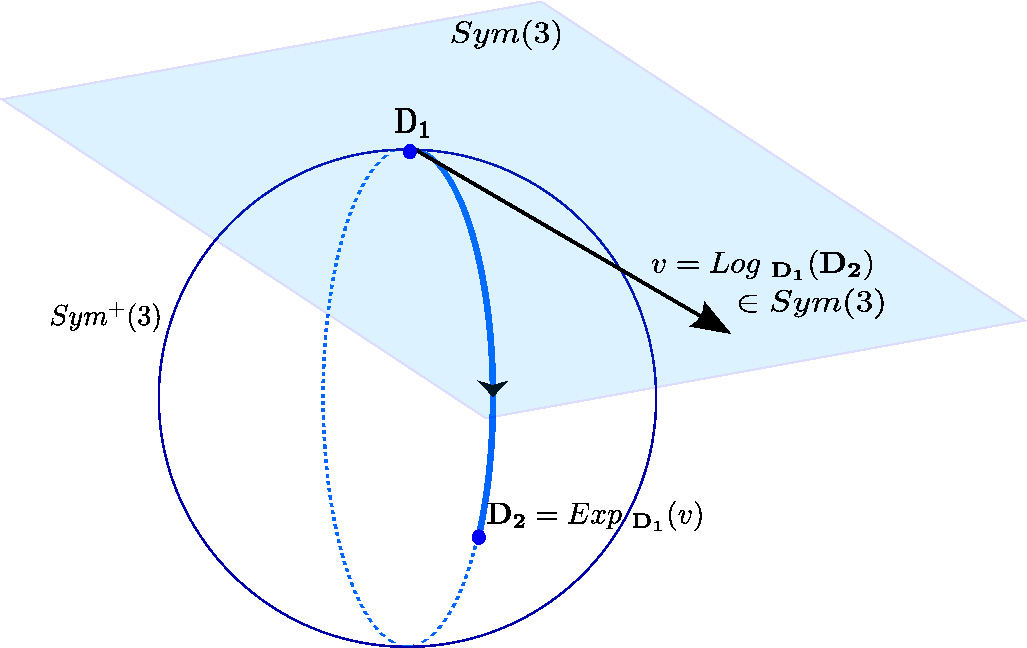
\includegraphics[scale=0.6]{Images/log_exp_map_sphere.pdf}
    \caption{\label{fig_log_exp_map} Illustration des cartes Riemanniennes logarithmique et exponentielle.}
\end{figure}

Cependant, à cause de la courbure de l'espace, l'implémentation de ces méthodes devient plus complexe et le temps d'exécution des calculs est considérablement plus long.
Dans l'optique d'éviter ces contraintes tout en conservant les propriétés théoriques convenables de l'espace Riemannien, 
de nouvelles métriques, appelées Log-Euclidiennes, sont proposées par~\cite{Arsigny2005,Arsigny2006} dans un cadre Riemanien.
Elles permettent de faire des \og aller-retours \fg entre un tenseur $\textbf{D}_\textbf{2}$ appartenant à l'espace des matrices symétriques définies positives $Sym^{+}(3)$ 
et son log-tenseur associé $Log_{\ \textbf{D}_\textbf{1}}(\textbf{D}_\textbf{2})$ de l'espace des matrices symétriques $Sym(3)$,
via le plan tangentiel au tenseur $\textbf{D}_\textbf{1}$ (voir le graphique en \figref{fig_log_exp_map}).
Par conséquent, l'enchainement suivant est rapide d'exécution, simple à implémenter et il garantit que le résultat est bien un tenseur de diffusion.
Le tenseur $\textbf{D}_\textbf{2}$ est projeté sur l'espace vectoriel associé au tenseur $\textbf{D}_\textbf{1}$.
Ensuite les métriques Euclidennes sont appliquées sur le log-tenseur $Log_{\ \textbf{D}_\textbf{1}}(\textbf{D}_\textbf{2})$ et $\textbf{D}_\textbf{1}$.
Enfin, le résultat peut être projeté de nouveau dans l'espace courbé.

Des travaux ont déjà évalué l'impact de telles métriques pour divers problèmes de traitements sur les tenseurs~\cite{Arsigny2006,Pasternak2010},
mais aucun ne précise la plus appropriée à utiliser, particulièrement dans le contexte de la comparaison de groupes.
%%%%%%%%%%%%%%%%%%%%%%%%%%%%%%%%%%%%%%%%%%%%%%%%%%%%%%%%%%%%%%%%%%%%%%%%%%%%%%%%%%%%%
\subsubsection{Problématique liée à l'étape du recalage}
C'est une étape fondamentale des pré-traitements en imagerie médicale. 
La comparaison de groupes nécessite une mise en correspondance spatiale des structures anatomiques afin de présenter les résultats en terme de regions neuro-anatomiques.
Cette étape permet de placer toutes les images des deux populations dans un même espace commun.

Nous pouvons décrire de manière très succincte le processus d'une telle étape.
Une étape de recalage consiste en une estimation du champ de déformations suivie par une application de ce champ aux images et d'une interpolation.
Plusieurs éléments composent la partie estimation de cette technique : des primitives à mettre en correspondance, un critère de similarité $f$, une transformation $t \in T$ ( $T$ étant le domaine des transformations), une méthode d'optimisation et bien évidemment deux images (une image source $I_s$ et une image de référence $I_r$). 

\begin{equation}
    \min_{t \in T} f(I_r, t(I_s) )
    \label{eq_recalage}
\end{equation}

Pour chaque élément de cette liste, il y a des sous-catégories : transformations globales ou locales, critère de similarité mono-modal ou multi-modal, type de primitives utilisées (voxels, surface, centre de gravité ...) ou encore le type de géométrie des transformations (rigide, affine et non-linéaire).
Dans la littérature, de nombreux travaux proposent des états de l'art complets sur l'étude du recalage en imagerie 
médicale~\cite{Noblet_PhD,Klein2009,Sotiras2013,Oliviera2014} dont certains sont plus spécifiques aux image du tenseur de diffusion~\cite{Zhang2007,Wang2011,Schwarz2014}.
Notre bibliographie s'est orientée autour de techniques de recalage sans structure particulière utilisant tous les voxels de nos images.
% image d'un pipeline 

Deux problématiques liées à l'étape du recalage appliqué aux images de tenseurs de diffusion se dégagent : l'interpolation et la ré-orientation des tenseurs.
En effet, dans le contexte du ITD, l'application d'un champ de transformations peut rencontrer de nombreuses difficultés, notamment dûes à la nature du tenseur de diffusion.\\

Premièrement, l'interpolation de deux tenseurs n'est pas évidente. 
Une interpolation linéaire de deux tenseurs avec une métrique Euclidienne de forme identique mais d'orientation perpendiculaire, 
un vertical et l'autre horizontal, produit une shpére et non pas un tenseur orienté à 45 degrés.
Ce problème rejoint celui présenté ci-dessus avec le paragraphe sur \og Problématique liée à la géométrie de l'espace des tenseurs \fg.
La \figref{fig_interpolation} illustre une interpolation linéaire des tenseurs avec trois métriques, une de chaque géométrie.\\
\begin{figure}[htpb]
    \centering
    \includegraphics[scale=0.8]{Images/interpolation_arsigny.pdf}
    \caption{\label{fig_interpolation} Illustration~\cite{Arsigny2005} d'interpolation linéaire des tenseurs avec des métriques différentes. \textbf{Haut} : métriques Euclidenne, \textbf{Milieu} : métrique Riemannienne. \textbf{Bas} : métrique Log-Euclidienne}
\end{figure}

Deuxièment, l'orientation des tenseurs après l'application de la transformation estimée peut se révéler particulièrement contraignante.
Dans l'image source transformée, les voxels prennent, par tranformée inverse, les tenseurs présents dans l'image source avant recalage.
Ces tenseurs ont une décomposition spectrale qui permet d'obtenir les axes de l'ellipsoïde ($\overset{\rightarrow}{e_1}$, $\overset{\rightarrow}{e_2}$, $\overset{\rightarrow}{e_3}$) 
et les valeurs propres associées ($\lambda_1$, $\lambda_2$, $\lambda_3$).
Cette décompostion n'a pas pris en compte les tranformations subies par l'image.
Ainsi dans l'image source tranformée, les tenseurs auront les même décompositions spectrales et par conséquent, les même orientations.
Prenons comme exemple de tranformation, illustré par la \figref{fig_reorientation}, un simple rotation de 45 degrés.
L'image (a) représente l'image source de base.
L'image (b) montre l'image (a) ayant subie une rotation de 45 degrés. 
Il est visible que les tenseurs n'ont pas suivi la rotation et reste tels qu'ils sont dans l'image (a).\\

\begin{figure}[htpb]
    \centering
    \includegraphics[scale=0.6]{Images/reorientation.pdf}
    \caption{\label{fig_reorientation} Illustration simple du problème de ré-orientation des tenseurs : rotation d'une image de tenseurs de diffusion de 45 degrés. (a) image d'origine, (b) image après application du champ de transformation,
    (c) image après application du champ de transformation et ré-orientation}
\end{figure}


\section{État de l'art en imagerie du tenseur de diffusion}
\label{etat_art}
En premier lieu, nous précisons que cet état de l'art ne s'intéresse qu'aux méthodes de détection de changements spécifiques
à l'imagerie du tenseur de diffusion et à la comparaison de groupes.
De nombreux articles et doctorats portent sur la détection de changements dans les divers autres domaines.
Pour une liste plus générale des références bibliographiques sur la détection de changements en imagerie de diffusion 
se réferrer au manuscrit de thèse d'Antoine Grigis \cite{Grigis_PhD}.\\

Les méthodes de détection peuvent être classées en trois grandes familles : 
les méthodes utilisant les indices scalaires dérivés du tenseur (FA ou MD), 
celles basées sur les vecteurs déduit du tenseur $vect(\mathbf{D})$
et enfin celles prenant en compte toute la matrice du tenseur $\mathbf{D}$.

La famille la plus grande est celle des méthodes basées sur les indices scalaires.
En effet, ces méthodes ne souffrent pas de problèmes de multi-dimensionnalité, ni de problèmes de variétés (voir \secref{problematiques}) : 
les indices scalaires commes leur nom l'indique sont des scalaires définis sur le domaine Euclidien.\\



Des modèles utilisant la matrice entière du tenseur ont aussi été développées \cite{Zhu2009, Schwartzman2010, Yuan2012, Bouchon2014, Kim2014} 
mais elles doivent faire face à l'incapacité du cadre euclidien pour tenir compte de la définie-positivité d'un tenseur de diffusion.\\

Comme expliqué dans la \secref{problematiques}, deux variétés avec des métriques prenant en compte la définie-positivité des tenseurs ont été proposées :
le Log-Euclidien \cite{Arsigny2006} et le domaine Riemanien \cite{Pennec1999}.\\

Quelques travaux ont déjà évalué l'impact des différentes métriques (Euclidiennes, Log-Euclidennes et Riemmaniennes) 
pour divers problèmes de traitement d'image \cite{Arsigny2006, Pasternak2010}, 
mais il n'y a toujours pas de consensus sur la variété la plus appropriée pour le traitement des tenseurs de diffusion, 
en particulier dans le contexte de comparaison de groupes.



\section{Pré-traitements}
\label{sec:preprocessing}
Cette section présente les trois pré-traitements implémentés dans la chaine de traitements : 
la correction des artefacts liés à l'acquisition,  l'estimation des tenseurs, le recalage qui permet de placer tous les sujets dans un même référentiel anatomique 
et enfin l'étape de filtrage permettant de lisser les observations afin de réduire le bruit et ainsi à améliorer les détections statistiques.

\subsection{Corrections des artefacts d'acquisition}
L'IRM de diffusion permet d'acquérir une série d'images pondérées en diffusion (DWI)
à partir de laquelle est estimée l'image du tenseur de diffusion (ITD).
Lors de l'acquisition, des artéfacts peuvent apparaître 
ce qui peut entraîner des distorsions importantes et compromettre les résultats des études.
Ils sont référencés dans la revue \cite{Jones2010}.
La plupart sont corrigés lors des pré-traitements afin d'obtenir des données 
les plus fiables possibles pour les analyses statistiques.
Pour cela, nous avons utilisé la méthode \og eddy\_current \fg de la librairie FSL\footnote{\url{http://fsl.fmrib.ox.ac.uk/fsl/}}.
% De plus, habituellement les gradients de diffusion sont normalisés mais nous avons eu un cas où ce n'était pas le cas. Nous avons alors dû corriger cette erreur et par défaut nous avons inclus une normalisation dans notre chaine de traitements. Cette opération par défaut est importante même si elle n'est que peu de fois exécutée car il suffit d'une série d'image avec des gradients de diffusion non normalisés pour fausser les résultats de la chaine de traitement.

\subsection{Estimation pondérée des tenseurs de diffusion}
La méthode classique d'estimation des tenseurs est celle des \og moindres carrés \fg.
Elle, ainsi que ses limites, sont décrites plus tôt dans le manuscrit (voir \chapref{Chapter1}).
Dans notre chaine de traitements, nous avons opté pour une méthode pondérée des moindres carrées proposé par \cite{Zhu2007} car
elle tient compte du fait que le bruit est un mélange de plusieurs bruits distribués différemment.
Les $n$ mesures pondérées en diffusion pour chaque voxel s'exprime sous la forme d'un triplet $(S_i, r_i, b_i)$ pour $i=1\ldots n$.
L'équation du signal acquis, et par conséquent bruité, s'écrit de la manière suivante après une transformée logarithmique pour linéariser le signal exponentiel : 
\begin{center}
    $log(S_i) = log(S_0) - b_i\textbf{r}_\textbf{i}^T\textbf{D}\textbf{r}_\textbf{i} + \eta_i$
\end{center}
Avec $S_i$ la $i^\text{ème}$ image pondérées en diffusion, $S_0$ l'image sans pondération, $b_i$ la b-valeur correspondante,
$\textbf{r}_\textbf{i} = (r_{i,1}, r_{i,2}, r_{i,3})^T$ le $i^\text{ème}$ vecteur de gradient de diffusion, $\eta_i$ le bruit lié à l'aquisition 
et enfin $\textbf{D}$ le tenseur de diffusion.
La méthode impose aux gradients de diffusion d'être distribués sur la sphère unité. 
Cela requière une normalisation au préalable des $n$ directions des gradients de diffusion pour qu'ils remplissent la condition suivante :
$\textbf{r}_\textbf{i}^{T}\textbf{r}_\textbf{i} = 1$.
L'estimation est initialisée par une méthode des moindres carrés classique suivie par plusieurs itérations $k_0 = 1\ldots 5$ d'une estimation par les moindres carrés pondérés.
Cette méthode est efficace et rapide d'autant plus que, comme démontré dans l'article \cite{Zhu2007}, 
une seule itération suffit lorsque le nombre de gradients de diffusion est égal ou supérieur à 30.
L'algorithme est détaillé ci-dessous par \algoref{algo:estimation_tenseur_2}.

\begin{center}
    \begin{minipage}[c]{0.9\textwidth}
	\begin{algorithm}[H]
	    \vspace*{0.5em}
	    \Data{
		$log(S_i) = z_i^T\theta + exp(-z_i^T\theta)\sigma\epsilon_i$ avec
		$z_i^T = (1, -b_i(r_{i,1}^2, 2r_{i,1}r_{i,2}, 2r_{i,1}r_{i,3}, r_{i,2}^2, 2r_{i,2}r_{i,3}, r_{i,3}^2))$
		et $\theta = (log(S_0), D_{11}, D_{12}, D_{13}, D_{22}, D_{23}, D_{33})$}\vspace*{1em}		
	    \Res{Estimation des 7 paramètres de $\theta$ : $\theta^{(k_0)} = (log(S_0), D_{11}, D_{12}, D_{13}, D_{22}, D_{23}, D_{33})$}
	    \Deb{
		initialisation $k = 0$ : $\hat{\theta}^{(k)} = ( \sum_{i=1}^{n} z_i z_i^T )^{-1} \sum_{i=1}^{n} z_i\ log(S_i)$\;\vspace*{1em}
		\Pour{$k_0$ itérations}{
		    $w_i^{(k)} = exp(2z_i^T\hat{\theta}^{(k)})$\;\vspace*{1em}
		    $\hat{\theta}^{(k+1)} = (\sum_{i=1}^{n} w_i^{(k)}z_iz_i^T)^{(-1)} \sum_{i=1}^{n} w_i^{(k)}z_i\ log(S_i)$\;
		}
	    }\vspace*{0.5em}
	    \caption{\label{algo:estimation_tenseur_2}Estimation du tenseur de diffusion par les moindres carrés pondérés}
	\end{algorithm}
    \end{minipage}
\end{center}

Pour mesurer la différence entre les méthodes des moindres carrées classiques et des moindres carrées pondérées, 
nous avons simulé un jeu de données de diffusion (type DWI) de synthèse basé sur les simulations introduites par \cite{Zhu2007} dans la section 3.1 de son article.
Nous avons effectué les deux estimations pour différentes valeurs du rapport signal sur bruit.
Pour chaque méthode, nous avons calculé l'erreur quadratique moyenne entre l'image de tenseurs d'origine et l'image de tenseurs estimée.
Nous avons mesuré une réduction d'erreur de 9\% en utilisant cette méthode comparée avec un moindres carrés classique.\\
{\color{red}ILLUSTRATIONS}

\subsection{Recalage}
L'état de l'art sur le sujet du recalage est disponible dans la \secref{problematiques} présentant les problématiques \ref{problematiques} en page \pageref{problematiques}.
Dans ce paragraphe, les trois méthodes de recalage utilisées dans la thèse seront exposés, ainsi que les raisons qui nous ont poussés à ces choix en particulier. 
Au cours de la thèse, nous nous sommes intéressé à l'influence que le recalage peut avoir sur les résultats des méthodes de détection. 
Et notamment aux fausses détections que peuvent engendrer une mauvaise ré-orientation ou une mauvaise estimation des déformations.
Pour répondre à la problèmatique présentée, nous avons sélectionné deux type des recalage différents : 
un recalage basé sur les cartes de scalaire avec une ré-orientation des tenseurs après l'application du champ de déformations 
et un recalage basé sur les cartes de tenseurs avec une ré-orientation des tenseurs directement intégrée de manière analytique dans la fonction de coût.

\subsubsection*{Recalage sur les images de FA}
La première méthode~\cite{Noblet2006} appartient au type de techniques le plus utilisée par la communauté en comparaison de groupes pour le ITD : 
les recalages qui estiment les champs de déformations sur les cartes de fraction d'anisotropie (FA) dérivées des images de tenseurs.

Cette méthode fonctionne en deux étapes.
Dans un premier temps, elle va estimer les transformations par la méthode des moindres carrées en se basant sur l'information mutuelle des images de FA.
Puis, dans un deuxième temps, sachant qu'il reste de petites distorsions anatomiques entre les images, 
un second recalage plus raffiné est effectué à l'aide d'une méthode non-rigide 
qui va estimer un modèle de déformation paramétrique multi-échelles toujours basé sur l'information mutuelle.
Ce recalage déformable peut être très puissant et compenser toutes les différences, de type anatomique ou pathologique, entre les images.
Pour éviter cela,~\cite{Noblet2006} propose d'imposer une contrainte de préservation de la topologie ainsi qu'un terme de régularisation.

Une fois les transformations finales estimées, elles sont appliquées sur les images de tenseurs en utilisant la méthode de 
Préservation de la Direction Principale~\cite{Alexander2001} pour ré-orienter les tenseurs correctement.

\subsubsection*{Recalage sur les images de tenseurs}
La deuxième technique appartient à la nouvelle génération qui estime les transformations directement sur les images de tenseurs.
Le défi du recalage d'images de tenseurs de diffusion est la multi-dimension des données et leur ré-orientation lors de l'application des transformations.
Une analyse comparative complète sur les différences entre 6 recalages basés scalaire et 2 basés tenseurs sont présentés par~\cite{Wang2011}.
Dans leur étude, la méthode \dtitk~\cite{Zhang2006, Zhang2007, Keihaninejad2013} montre les meilleurs résultats d'après les trois critères d'évaluation qu'ils proposent.
Les auteurs concluent en recommandant l'algorithme \dtitk par rapport aux autres méthodes déformables basées sur les tenseurs.
Cet outils de recalage est disponible en ligne\footnote{\url{http://www.nitrc.org/projects/dtitk}}.\\

La méthode \dtitk permet d'estimer les 12 paramètres d'une transformation affine $\textbf{p}$.
Cette estimation est faite morceau par morceau ce qui rend le champ des transformations globales non-linéaire.
L'expression de la transformation affine $F$ est décomposée en 3 matrices de base appliquées au voxel $x$ : 
\begin{equation}
    F(x) = (QS)x + T
    \label{fct_affine_dtitk}
\end{equation}
avec $T$ une matrice de translation, $S$ une matrice de pure déformation et $Q$ une matrice de pure rotation.
L'application de cette matrice $Q$ permet de ré-orienter un tenseur $\textbf{D}$ : $Q\textbf{D}Q^t$~\cite{Alexander2001}.
La méthode définit une fonction de coût $O$ qui intègre de façon explicite cette ré-orientation des tenseurs dans son expression :
\begin{equation}
    O(\textbf{p}) = \int_{\mathcal{R}^3} \|\textbf{D}_s((QS)x + T) - Q\textbf{D}_rQ^t\|^2dx
    \label{fct_cout_dtitk}
\end{equation}
avec $\textbf{D}_r$ et $\textbf{D}_s$ respectivement le tenseur de référence et le tenseur source à déformer.\\

De plus, la méthode \dtitk estime les 12 paramètres $\textbf{p}$ de la transformation affine morceau par morceau sur des régions de taille égale $\Omega_i$
en imposant une contrainte de continuité inter-régions.
Pour cela, l'algorithme essaie de minimiser la différence entre les transformations affines de deux régions.
\begin{equation}
    \int_{\Omega_i\bigcap\Omega_j} \|F_i(x) - F_j(x)\|dx
    \label{fct_cont_dtitk}
\end{equation}
L'expression analytique des équations \eqref{fct_cout_dtitk},\eqref{fct_cont_dtitk} permet une résolution du problème par les gradients conjugués.\\

\begin{figure}[htpb]
    \centering
    \includegraphics[scale=0.7]{Images/dtitk_hierarchie.pdf}
    \caption{\label{fig_dtitk_hierarchie}Illustration de l'approche hiérarchique de l'algorithme \dtitk.
    (a) est la représentation du partage initial ($n=2$) grossier de l'image avec les estimations des transformations sur chaque région.
    (b) est la représentation au niveau supérieur ($n=4$) avec l'estimation des transformations initialisée par les transformations du niveau inférieur.}
\end{figure}
Les transformations finales sont estimées par une approche hiérarchique illustrée par la \figref{fig_dtitk_hierarchie}.
L'algorithme estime les premières transformations $F_i^{n}$ sur une image découpée grossièrement ($n=4$ régions sur chaque côté de l'image 3D).
Par la suite, il raffine son estimation en partageant plus finement l'image ($n=8, 16$) et en initialisant les transformations avec celles du niveau inférieures.

\subsubsection*{Recalage sur les images d'IRM de T1}
Dans son article, \cite{Tustison2014} met en avant un fait important :
estimer les tranformations du recalage sur les même cartes de données sur lesquelles l'analyse statistique
sera effectuée, revient à introduire un biais dans le modèle favorisant les détections.
Il appelle ce phénomène, \og circularity bias \fg et cela se traduit pas une augmentation générale des p-valeurs.
Pour supprimer ce biais, \cite{Tustison2014} conseille d'éviter les recalage basés sur le même jeu de données 
que celui utilisé pour l'analyse statistique lors de la compraison de groupes.
À la place, un recalage en deux étapes est recommandé. 
Dans un premier temps, un recalage multi-modal et intra-individu est effectué entre les cartes de FA vers les cartes d'IRM de T1.
Il est suivi, dans un deuxième temps, par un recalage sur les cartes T1 inter-individus combinant une méthode affine et une méthode non-linéaire~\cite{Noblet2006}.


\subsection{Filtrage}


Après l'étape de recalage, il est recommandé d'utiliser un filtre sur les images de tenseurs dans le but de lisser les observations, de réduire le bruit présent et ainsi contribuer à améliorer les détections statistiques.

    %%%%%%%%%%%%%%%%%%%%%%%%%%%%%%%%%%%%%%%%%%%%
% Chapitre 4
%%%%%%%%%%%%%%%%%%%%%%%%%%%%%%%%%%%%%%%%%%%%

\chapter{Méthode linéaire}
\label{Chapter4}

    %%%%%%%%%%%%%%%%%%%%%%%%%%%%%%%%%%%%%%%%%%%%
% Chapitre 5
%%%%%%%%%%%%%%%%%%%%%%%%%%%%%%%%%%%%%%%%%%%%

\chapter{Variétés non linéaires}
\label{Chapter5}

% \minitoc

%----------------------------------------------------------------------------------------

\section{Problématique des métriques euclidiennes}
% \lipsum[22-26]
\section{Géométrie riemanienne}
% \lipsum[22-26]
\subsection{Principe}
\subsection{État de l'art des régressions sur cette variété}
\subsection{Méthode du "Multivariate General Linear Models"}
\subsubsection{Description de la méthode}
\subsubsection{Test statistique}

\section{Géométrie log-euclidienne}
\subsection{Principe}
\subsection{Application dans le cadre GLM-DT}


% \section{Conclusion partielle}

    %%%%%%%%%%%%%%%%%%%%%%%%%%%%%%%%%%%%%%%%%%%%
% Chapitre 6
%%%%%%%%%%%%%%%%%%%%%%%%%%%%%%%%%%%%%%%%%%%%

\chapter{Caractérisation des changements}
\label{Chapter6}

Le \chapref{Chapter4} présente des méthodes de détection de changements entre deux populations de tenseurs.
Ces méthodes de comparaison de groupes permettent de détecter les régions pour lesquelles la forme des tenseurs de diffusion diffère 
significativement d'une population à l'autre, sans toutefois donner d'information sur la nature des changements observés.
Ainsi, une méthode complémentaire est proposée, permettant de caractériser a posteriori les changements détectés en termes de
modification de la Fraction d'Anisotropie (FA), Diffusion Moyenne (DM), Diffusion Radiale (DR) ou Diffusion
Axiale (DA), afin de rendre l'interprétation des résultats plus aisée pour le Neurologue.\\

% \minitoc

%----------------------------------------------------------------------------------------

\section{Post-traitement général}
Les cartes de \textit{p-valeurs} obtenues en sortie des méthodes de détection des changements sont dites \og brutes \fg,
c'est-à-dire sans avoir subies de transformations quelconques pour améliorer les détections.
Nous les appellerons par la suite \og cartes primaires \fg.
Il est possible d'appliquer, de manière systématique, des corrections statistiques et morphologiques à ces cartes.
Le post-traitement général présenté dans cette section est effectué en deux étapes : 
une correction statistique des cartes de \textit{p-valeurs} suivie d'une correction sur la topologie des détections.
Après ces corrections, la carte de résultats est appelée \og carte corrigée \fg.

\subsection{Correction statistique des cartes de p-valeurs}
Positionnons-nous dans le cas de la compraison de groupes en imagerie médicale.
Nous avons $N$ images-sujets comportant $V$ voxels chacune.
Le \mlg va réduire pour chaque voxel les $N$ informations en $K$ régresseurs et 
le test statistique va mesurer l'effet d'un de ces régresseurs pour chaque voxel.
En sortie, nous obtenons une carte de $V$ \textit{p-valeurs} (carte primaire de détection).
Durant ce processus, le test d'hypothèse \eqref{test_stat} est effectué $V$ fois.
Ces $V$ tests sont indépendants et pour chacun le niveau de signification est nommé $\alpha_{test}$. 
Il correspond à la probabilité de rejeter l'hypothèse nulle $\mathcal{H}_0$ alors qu'elle est vraie, 
ou encore à la probabilité de détecter un Faux Positif.
Sur ces $V$ tests, nous connaissons le nombre $A$ de décisions acceptant l'hypothèse $\mathcal{H}_0$ et le nombre $R$ la rejetant ($V=A+R$).
Trois cas sont possibles : \\
\begin{itemize}
    \item Sans aucune correction, un pourcentage $\alpha_{test}$ des $V$ voxels sont des Faux Positifs.\\
    
    \item Le premier type de correction sert à contrôler le nombre de Faux Positifs parmi le $V$ voxels.
    C'est la méthode de Bonferroni \cite{Abdi2007} (ou encore en anglais \textit{Family Wise Error Rate} FWER).
    Les $V$ tests sont indépendants donc la probabilité d'accepter l'hypothèse nulle $\mathcal{H}_0$ pour cette famille de test est : $(1-\alpha_{test})^V$.
    Il en découle directement la probabilité de rejeter $\mathcal{H}_0$ pour la famille de test : $\alpha_{famille} = 1 - (1-\alpha_{test})^V$.
    Par exemple, si $V=100$ et $\alpha_{test} =0.05$ alors $\alpha_{famille}=0,00592$.
    Pour une image classique du tenseur de diffusion avec une taille de $128\time128\time41$, nous avons $V=671744$ voxels.
    Alors la probabilité $\alpha_{famille}$ devient très petite, rendant la correction trop stricte.\\
    
    \item La deuxième méthode de correction va contrôler le nombre de Faux Positifs $FPos$ parmi les $R$ détections \cite{Benjamini1995, Benjamini2001}
    (en anglais \textit{False Discovery Rate} FDR).
    Il définit un taux de Faux Positif $taux_{FPos}$ et exprime le FDR comme l'espérance de ce taux devant être inférieur au niveau de signification $\alpha_{test}$ :
    \begin{align}
        taux_{FPos} &= \left\{ \begin{array}{lr} \frac{FPos}{R} & : R > 0\\ 0 & : sinon \end{array} \right.\\
        FDR &= E\left[taux_{FPos} \right] < \alpha_{test}
    \end{align}
    La procédure consiste à classer les $R$ \textit{p-valeurs} : $p_1 \leq p_2 \leq \dots p_R$ par ordre croissant.
    Et à rejeter les $k$ \textit{p-valeurs} (parmi les $R$) qui vérifient :
    \begin{equation}
        p_i \leq \frac{i}{V}\alpha_{test} 
    \end{equation}
    Avec cette correction, seuls $\alpha_{test}$ voxels sur les $R$ sont des fausses alarmes (Faux Positifs).
    Pour notre chaine de traitements, nous avons choisi cette correction.
\end{itemize}


\subsection{Composantes connexes}
La correction statistique permet de contrôler le taux de Faux Positifs sur l'image entière
mais ne fait aucune intervention par rapport à la morphologie des zones détectées.
Physiquement, il est facile de comprendre que les détections de voxels isolés ou encore des agrégats de voxels de toutes petites tailles, ne sont pas représentatifs d'une lésion 
car elles sont, de manière générale, plus étendues sur la substance blanche.
Par exemple, pour une image de résolution $1.8\time1.8\time3.5 mm^3$, une détection isolée (1 seule voxel) corresponderait à une lésion d'environ $12 mm^3$.
Ces détections sont souvent attribuées à de Faux Positifs.
Par la suite, il est préférable de ne conserver que les agrégats dont la taille est supérieure à celle fixée par l'utilisateur (voir \figref{etape_carac_1}).
Pour cela, nous utilisons la méthode des composantes connexes.
Ce sont des opérateurs de morphologie mathématique qui servent, généralement, d'outils de filtrage et de segmentation.

\begin{figure}[ht]
  \centering
  \includegraphics[scale=0.5]{Images/etape_carac_1.pdf}
  \caption{\label{etape_carac_1}Illustration du post-traitement général.}
\end{figure}


\section{Caractérisation des zones détectées}
Les méthode de comparaison de groupes basées sur les tenseurs sont des extension du \mlg.
Avec le test de Fisher introduit au \chapref{Chapter4}, une carte de \textit{p-valeurs} est obtenue.
Elle est ensuite corrigée par la méthode du False Discovery Rate (FDR), puis seuillée à un seuil de 5\%.
Cette approche permet d'identifier les régions atteintes par la pathologie, sans apporter d'information sur la nature et le sens des changements détectés.
Cette section présente une méthode de post-traitement pour pallier à la problématique des méthodes de détection.
Elle consiste à caractériser les détections obtenues avec les méthodes du \chapref{Chapter4}.


\subsection{Description de la méthode de caractérisation}
Les méthodes de comparaison de groupes permettent de prendre en compte toute l'information contenue dans les tenseurs sous différentes hypothèses
(homoscédasticité et hétéroscédasticité).
Pour chaque méthode, des régresseurs associé à chaque élément du tenseur, sont estimés au sens des moindres carrés.
Ensuite, un test statistique de Fisher est utilisé pour tester la significativité des effets de ces regresseurs dans les modèles.

La première étape (voir \figref{etape_carac_1}) de la caractérisation des changements consiste à corriger les cartes de détection par la méthode du FDR,
puis à étiqueter les composantes connexes de la carte des détections seuillée 
et à ne conserver que celles dont la taille est supérieure à un seuil fixé par l'utilisateur. 
Cette étape correspond aux opérations du post-traitement général.

\begin{figure}[ht]
    \centering
    \includegraphics[scale=0.6]{Images/etape_carac_2.pdf}
    \caption{\label{etape_carac_2}Illustration de la deuxième étape de la caractérisation.}
\end{figure}
La deuxième étape (voir \figref{etape_carac_2}) consiste, sur chaque région et pour chaque sujet, à calculer les valeurs
moyennes des différents indices scalaires (\fa (FA), \md (DM), \dr (DR) et \da (DA)) et à comparer indépendemment chacune de ces quantités grâce à
un \mlg, en utilisant les même covariables que précédemment.

\begin{figure}[ht]
    \centering
    \includegraphics[scale=0.6]{Images/etape_carac_3.pdf}
    \caption{\label{etape_carac_3}Illustration de la troisième étape de la caractérisation.}
\end{figure}
Un test de Student, ou encore T-test, est réalisé pour chaque agrégat, afin d'identifier le sens du changement détecté (voir \figref{etape_carac_3}).
L'hypothèse nulle $\mathcal{H}_0$ vérifie $c^t \hat{B} =0 \text{ avec } c \in \mathbb{R}^{k}$ 
le vecteur de constraste permettant de faire une combinaison linéaire des régresseurs $\hat{B}$.
\begin{equation}
    t = \frac{c^t\hat{B}}{\sqrt{c^t\hat{\Sigma}c}} \sim T_{d=N-K}
\end{equation}
Contrairement au test statistique utilisé \eqref{test_stat} pour les méthodes de détection,
il est alors possible de tester l'équalité entre deux régresseurs en mettant à $1$ et $-1$ les contrastes associés aux deux régresseurs à l'étude et tous les autres contrastes à $0$.
Ou encore, nous pouvons tester si un régresseur n'a pas d'effet sur le modèle en mettant le constraste associé à $1$ et les autres à $0$ pour, par exemple, étudier la corrélation supposée entre un score clinique et les observations.

Il faut noter une différence par rapport au cadre statistique précédent.
Dans le cas de ce test, pour la comparaison de groupes, il faut deux variables explicatives pour les deux groupe $\{x_1, x_2\}$ 
afin d'estimer un régresseur représentant le premier groupe et un deuxième pour l'autre groupe.


\subsection{Format de présentation des résultats}
La liste de ces régions est présentée au médecin en respectant l'ordre suivant dans les indices scalaire : DA:\da, DR:\dr, DM:\md, FA:\fa.
Seules les régions ayant conduit à au moins un test significatif au seuil de 5\% sont conservées. 
Cette liste précise le sens de modification du test à l'aide de deux symboles : ($+$) pour une augmentation et ($-$) pour une diminution, 
ainsi que le niveau de signification : ($n.s.$) pour un résultats non significatif.
Un exemple fictif, correspondant au schéma de la \figref{etape_carac_3}, est donné par le \tabref{ex_caracterisation}.
Les trois agrégats violet, vert et rouge correspondent respectivement aux numéros {\color{purple}1}, {\color{green}2} et {\color{red}3}.

\begin{table}[ht]
\centering
\begin{tabular}{|D{2cm}|D{1cm}|D{1cm}|D{1cm}|D{1cm}|}
      \hline
      \textbf{Agrégats} & \textbf{DA} & \textbf{DR} & \textbf{DM }& \textbf{FA} \tabularnewline
      \hline
      {\color{purple}1} & $-$ & $n.s.$ & $-$ & $-$\tabularnewline
      {\color{green}2} & $n.s.$ & $+$ & $+$ & $-$\tabularnewline
      {\color{red}3} & $-$ & $-$ & $-$ & $n.s.$\tabularnewline
      \hline
  \end{tabular}
  \caption{\label{ex_caracterisation}Exemple de liste présentant les résultats de la caractérisation.}
\end{table}

Dans la littérature \cite{Harsan2006}, deux types de modification ont été reliés à des phénomènes biologiques provoqués 
par des pathologies dégénératives du système nerveux central chez l'homme :\\
\begin{itemize}
    \item une diminution de la \da peut représenter une modification axonale comme une réduction du diamètre de l'axone.
    Cela engendrera aussi une diminution de la \md et de la Fraction d'Anisotropie.
    Dans ce cas de figure, les changements détectés en \dr ne sont pas représentatifs de la modification et nous admettons qu'ils peuvent être $-/+/n.s.$.
    La combinaison des symboles est : \{$-$, $(-/+/n.s.)$, $-$, $-$\}\\
    \item une augmentation de la \dr peut représenter une dégradation de la couche de myéline.
    Nous parlons alors de démyélinisation.
    Cela entraine une augmentation de la \md et une diminution de la Fraction d'Anisotropie.
    Dans ce cas là, les modifications détectées pour l'indice scalaire \da ne correspondent pas à des cas réels et les trois symboles $-/+/n.s.$ peuvent leur être attribués.
    La combinaison des symboles est : \{$(-/+/n.s.)$, $+$, $+$, $-$\}\\
\end{itemize}

Certaines combinaisons de symboles, par exemple \{$-$, $-$, $-$, $n.s.$\} ou encore \{$-$, $-$, $-$, $+$\}, 
représentent des modifications qui ne peuvent être associées avec des cas réels.
Deux explications permettent de comprendre ces résultats.
Tout d'abord, les changements détectés correspondent à une modification de l'orientation de la diffusion ce qui est impossible à détecter avec les valeurs scalaires.
Ensuite, il est possibile que plusieurs modifications différentes soient présentes dans l'agrégat et en faisant la moyenne des valeurs scalaires, 
les différents changements se compensent les uns aux autres.


\begin{figure}[ht]
    \centering
    \includegraphics[width=1\textwidth]{Images/pipeline.pdf}
\end{figure}

    
      % partie 3
    \part{Simulations et validations}
    \label{Part3}
    %%%%%%%%%%%%%%%%%%%%%%%%%%%%%%%%%%%%%%%%%%%%
% Chapitre 6
%%%%%%%%%%%%%%%%%%%%%%%%%%%%%%%%%%%%%%%%%%%%

\chapter{Cohortes de données utilisées}
\label{Chapter7} 

    %%%%%%%%%%%%%%%%%%%%%%%%%%%%%%%%%%%%%%%%%%%%
% Chapitre 8
%%%%%%%%%%%%%%%%%%%%%%%%%%%%%%%%%%%%%%%%%%%%

\chapter{Évaluation de la méthode GLM-DT dans un cadre statistique Euclidien}
\label{Chapter8}

    %%%%%%%%%%%%%%%%%%%%%%%%%%%%%%%%%%%%%%%%%%%%
% Chapitre 9
%%%%%%%%%%%%%%%%%%%%%%%%%%%%%%%%%%%%%%%%%%%%

\chapter{Influence du cadre statistique sur des méthodes basées tenseurs}
\label{Chapter9}



% \minitoc

%----------------------------------------------------------------------------------------

\section{Évaluation de la variété géométrique utilisée}
La \figref{fig:res_manifold} présente les différents résultats obtenus pour la comparaison entre les métriques des variétés Euclidienne, Log-Euclidienne et Riemmanienne.
D'une part, ils mettent en évidence que les performances de ces méthodes varient suivant le type de lésion simulée.
La méthode \textit{GLM-DT} surpasse les deux autres pour détecter une diminution de la diffusion longitudinale.
D'autre part, les méthodes \textit{GLM-LOG-DT} et \textit{MGLM-DT} montrent des résultats légèrement supérieurs 
pour détecter des lésions produits par une augmentation de la diffusion radiale.
Il faut aussi noter que ces trois méthodes présentent des performances similaires pour la détection des deux autres types de lésions 
(une modification de l'orientation de la diffusion et une augmentation de la diffusion moyenne).
Enfin, nous remarquons que les méthodes utilisant des métriques Log-Euclidienne et Riemmanienne mènent à des résultats particulièrement similaires.

\begin{figure*}[t]
    \centering
    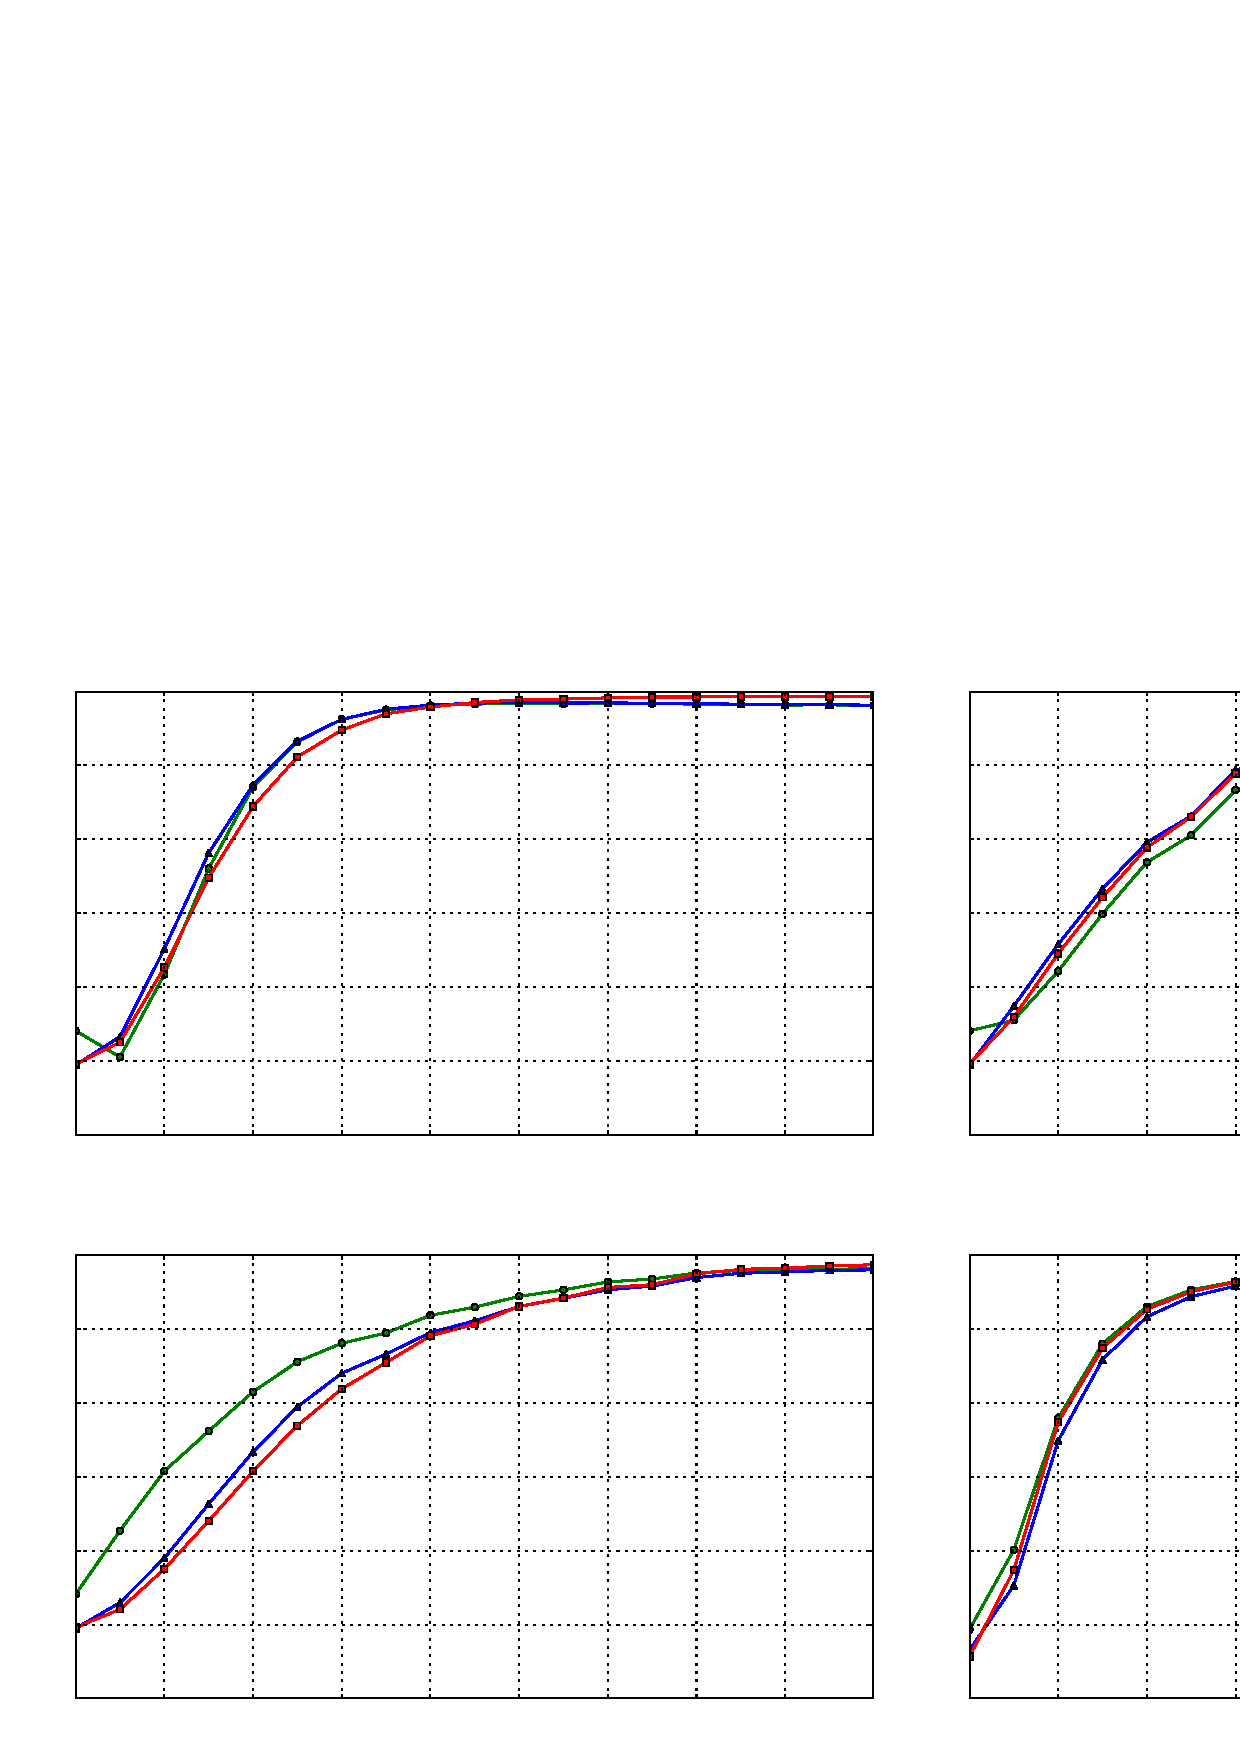
\includegraphics[width=1\textwidth]{Images/AUC_frameworks_gaussian8_fr.pdf}
    \caption{\label{fig:res_manifold} Influence de la variété géométrique ({\color{green} $\bullet$ = GLM-DT},  {\color{blue} $\blacktriangle$ = GLM-LOG-DT}, {\color{red} $\blacksquare$ = MGLM-DT}).}
\end{figure*}


\section{Discussion}

In the literature, a few works have already evaluated the impact of the Euclidean, Log-Euclidean and affine invariant-Riemannian metrics
 for various images processing problems \cite{Arsigny2006, Pasternak2010} but there is still no consensus on the most appropriate manifold for handling diffusion tensors, 
especially in the context of group comparison.
Some papers prone the use of  Log-Euclidean or Riemannian metrics for conducting DT-MRI group comparison \cite{Zhu2009, Schwartzman2010, Yuan2012, Kim2014}.
Some other papers claim that these metrics are not superior \cite{Whitcher2007} or even inferior \cite{Pasternak2010} to the Euclidean one. In their comparison between Euclidean
and Log-Euclidean metrics, Whitcher \textit{et al}  \cite{Whitcher2007} conclude that there is no reason to prefer the log-Euclidean distance and that
applying matrix logarithms to diffusion tensors tends to reduce the group difference observed in Euclidean space.
Moreover, both theoretic analysis and experimental results reported in \cite{Pasternak2010} support that the Euclidean metric is more appropriate than an affine-invariant metric for the analysis of diffusion coefficients and tensors.

Our experimental results on simulated lesions highlight that all metrics can efficiently detect every kind of lesions,
with performance varying for each framework according to the kind of simulated change.
The results on the real database confirm the good ability of the three metrics to detect the regions
involved in the NMO, without exhibiting any significant difference between the detection maps.
Regarding the computational burden (\tabref{tab:cpu_time}), 
the typical computation time for conducting the statistical analysis of the NMO database on a standard workstation 
is about 2 min for the Euclidean and Log-Euclidean approaches as compared to about 80 hours for the Riemannian framework. 
This time gap may probably be reduced by optimizing the implementation of the Riemannian framework\footnote{\url{https://www.nitrc.org/projects/riem\_mglm}},
for instance by rewriting the MATLAB code in C++ language.
But in any case, the Riemannian framework would still be much more computationally intensive than the Euclidean and Log-Euclidean approaches.


\begin{table}[htbp]
\centering
\begin{tabular}{|D{4cm}|D{4cm}|}
      \hline
      \textbf{Méthodes} & \textbf{Temps d'exécution ($s$)} \tabularnewline
      \hline
      GLM-FA & 135 \tabularnewline
      GLM-MD & 135 \tabularnewline
      GLM-DT & 135 \tabularnewline
      GLM-LOG-DT & 148 \tabularnewline
      MGLM-DT & 253392 \tabularnewline
      \hline
  \end{tabular}
  \caption{\label{tab:cpu_time} Temps d'exécution en $s$ pour les analyses statistiques de la base NMO.}
\end{table}

In conclusion, this study suggests that, despite the mathematical elegance offered by the Riemannian framework, its superiority on both simulated and real clinical data could not be demonstrated compared to the Euclidean and Log-Euclidean frameworks. 
For a similar performance, these two latter methods present the advantage to be easily implementable and computationally effective. This conclusion is of course limited to the scope of the present application. 

    %%%%%%%%%%%%%%%%%%%%%%%%%%%%%%%%%%%%%%%%%%%%
% Chapitre 10
%%%%%%%%%%%%%%%%%%%%%%%%%%%%%%%%%%%%%%%%%%%%

\chapter{Influence des pré-traitements pour une comparaison de groupes}
\label{Chapter10}



% \minitoc

%----------------------------------------------------------------------------------------


\section{Recalage}
\section{Filtrage}
    %%%%%%%%%%%%%%%%%%%%%%%%%%%%%%%%%%%%%%%%%%%%
% Chapitre 11
%%%%%%%%%%%%%%%%%%%%%%%%%%%%%%%%%%%%%%%%%%%%

\chapter{Contributions aux neurosciences}
\label{Chapter11}



% \minitoc

%----------------------------------------------------------------------------------------

\section{Sur la base de patients atteints de NMO}

\subsection{Résultats des méthodes linéaires}




\section{Sur la base de patients atteints de DLB}
\subsection{Comparaison de patients au stade prodomal avec des témoins}
\subsection{Étude sur les hallucinations dans le maladie à corps de Lewy}



    
    \part{Conclusion}
    \label{Conclu}
    
    
    \pagestyle{introduction}
      % bibliographie
    \biblio{Bibliography}
    \label{Biblio}
    \bibliographystyle{ieeetr}
    \bibliography{Bibliography/bibliography}
%     \addstarredchapter{\textsc{Bibliographie}}
    \markboth{\textsc{Bibliography}}{}
    
    \backmatter
    \listoffigures
%     \addstarredchapter{Liste des figures}
    \listoftables
%     \addstarredchapter{Liste des tableaux}
%     
%     \appendix


\end{document}
